\chapter{Multiresolution Sinusoidal Neural Networks}

In this chapter, we introduce a novel neural network architecture designed to encode signals at multiple scales. Our objective is to achieve a continuous and compact representation of scalar and vector fields, which can be applied to model images, shapes, and other complex media objects, either as explicit attributes of space-time coordinates or as level sets of implicit functions.

We initially focus on representing one-dimensional signals using sinusoidal neural networks. This approach allows us to experiment on the control of signal frequencies, visualize them through their Fast Fourier Transform (FFT) plots, and validate our results against classical sampling theory.

Our architecture builds upon the Sinusoidal Representation Networks (SIREN) framework (\cite{sitzmann2019siren}), known for its ability to learn high-frequency signal details efficiently and model signal derivatives. We deeply investigate the network's initialization, exploring the interplay between its hyperparameters, the inherent frequencies of a signal, and the frequencies the network learns.

For the multiresolution approach, we leverage classical structures of image and signal processing, such as Gaussian and Laplacian Pyramids. We use these ideas to develop a framework to train a multi-stage neural network using multiresolution structures in an efficient way. \red{Finally, we demonstrate that our model can achieve a comparable reconstruction quality to a simple SIREN model with the same number of parameters, while encoding multiple levels of detail. Esta frase deve ser movida para o capítulo seguinte, de aplicações em imagens. A conclusão desta parte será finalizada quando este capítulo estiver completo.}


\section{Related Works}

Our focus lies on signals as media objects, usually represented by functions in one, two, and three dimensions. \cite{tancik2020fourfeat} demonstrated, both theoretically and empirically, that standard Multilayer Perceptrons (MLPs) struggle to learn high frequencies in such domains, which are considered low-dimensional domains for machine learning applications. They proposed using Fourier feature mapping to transform input coordinates into a higher-dimensional spectral feature space before processing them through the network. This enables coordinate-based MLPs to effectively capture high-frequency content in low-dimensional signals, overcoming this \textit{spectral bias} (\cite{rahaman2018spectral}).

Sinusoidal neural networks represent a class of coordinate-based networks that employs the sine function as their activation function. They serve as a bridge between spatial and spectral domains due to the close relationship between the sine function and the Fourier basis. The first layer of a sinusoidal neural network projects the signal into spectral space, while the last layer reconstructs the signal from a dictionary of spectral atoms. This characteristic allows them to naturally overcome the spectral bias of regular MLPs. However, these sinusoidal neural networks have been regarded as difficult to train \cite{taming2017}. To address this issue, Sitzmann et al. \cite{sitzmann2019siren} proposed SIREN, a sinusoidal network for signal representation. One of its key contributions is an initialization scheme that ensures stability and convergence, enabling the modeling of fine details consistent with the signal’s frequency content.

The challenge in training sinusoidal neural networks comes in part from the composition of sinusoidal functions, which can generate multiple new and higher frequencies. \cite{novello2022understanding} studied sinusoidal MLPs by expanding them as harmonic sums, demonstrating how numerous new frequencies are expressed as integer linear combinations of the input frequencies. This work provides theoretical justification for sinusoidal MLPs compactness property and contributes to a better understanding of these networks’ behavior.

A simpler form of sinusoidal network is the Multiplicative Filter Network (MFN) \cite{fathony2020multiplicative}, which is equivalent to a shallow sinusoidal MLP. \cite{bacon2021} introduced the Band-Limited Coordinate Network (BACON), an MFN that produces intermediate outputs with an analytically specified spectral bandwidth, achieving multiresolution representations of underlying signals. While its structure allows BACON to be expressed as a linear combinations of sines, avoiding the composition of sines present in deep sinusoidal MLPs, it creates multiresolution representations by truncating the frequency spectra of the signals at a specific value. This approach produces ringing artifacts in some levels of detail, and becomes evident when we look at the Fourier transform of images reconstructed using this network (see Chapter \ref{ch:imaging}).

The ability to control frequency bands in representation is closely tied to the capability of adaptively reconstructing signals at multiple detail levels. \citet{mueller2022instant} developed a multiresolution neural network architecture based on hash encoding, while \citet{martel2021acorn} designed an adaptive coordinate network for neural signals.

In this context, we introduce \textit{Multiresolution Sinusoidal Neural Networks} (MR-Net) \cite{paz2022,paz2023mr} based on classical signal multiresolution representations. Our results in imaging applications, discussed in Chapter \ref{ch:imaging}, demonstrate that MR-Net outperforms the previous state-of-the-art technique, BACON, while utilizing a smaller number of parameters.


\section{Frequency Initialization}

The correct initialization of sinusoidal neural networks is crucial for having stability during training and convergence to the expected result. According to \cite{sitzmann2019siren}, a SIREN model must be initialized so that for a uniform input in $[-1, 1]$ the outputs of each hidden layer before the sine nonlinearity are standard normal distributed. 

% such that, for a uniform input in \([-1, 1]\), the outputs of each hidden layer before applying the sine nonlinearity are normally distributed with a mean of zero and a standard deviation of one. 

Moreover, the authors of SIREN propose to initialize the first layer of the network so that the sine function $\sin(\omega_0 \cdot W x + b)$ spans multiple periods over $[-1, 1]$. They introduce $\omega_0$ as a hyperparameter that could be adjusted to each signal, while $W$ and $b$ are the weights and biases of a layer in the network. For the examples presented in their work, they used a fixed $\omega_0=30$ and found it to work well empirically, but they did not dive deeper on the \emph{why}.

% The authors of SIREN suggest initializing the first layer of the network to ensure that the sine function \(\sin(\omega_0 \cdot Wx + b)\) spans multiple periods over \([-1, 1]\). They introduce \(\omega_0\) as a hyperparameter that can be adjusted for each signal. Empirically, they found a fixed \(\omega_0 = 30\) to work well, although they do not delve into the underlying reasons.

% In this section, we show how the choice of $\omega_0$  impacts the frequencies learned by the network, the speed of the training and even if it will converge to a reasonable result or collapse into noise. The hyperparameter $\omega_0$ is directly related to the interval of frequencies used to initialize the first layer of the network, determining the set of the spectral atoms where the signal will be projected. This same hyperparameter is also applied on the initialization of the hidden layers as the authors argue it boosts the gradients during the training and accelerates the convergence. However, in the hidden layers, it is basically used as pre-conditioner, a numeral trick, since the implementation multiplies by $\omega_0$ and also divides by this same value. We propose to call this hyperparameter in the hidden layers by $\omega_h$, and keep $\omega_0$ only for the first layer.

In this section, we examine how the choice of \(\omega_0\) impacts the frequencies learned by the network, \red{the speed of training}, and whether the network will converge to a reasonable result or collapse into noise. We show that the hyperparameter \(\omega_0\) directly influences the range of frequencies used to initialize the first layer of the network, thus determining the set of spectral atoms onto which the signal will be projected. This hyperparameter is also applied to the initialization of the hidden layers, as the authors argue that it boosts gradients during training and accelerates convergence. However, in the hidden layers, \(\omega_0\) functions primarily as a pre-conditioner, a numerical trick, since the implementation multiplies the weights by \(\omega_0\) and then divides them by the same value. To clarify this distinction, we propose referring to the hyperparameter in the hidden layers as \(\omega_h\), reserving \(\omega_0\) exclusively for the first layer.

By understanding and adjusting \(\omega_0\), we aim to optimize the training process of sinusoidal neural networks and develop a multiresolution architecture with them.


\subsection{Isolating Frequencies}

A shallow network with just one layer of sinusoidal activation functions can filter a signal by band-limiting its frequency content. Thus, it provides a tool for controlling the level of detail of the output signal. This conclusion is natural since the resulting signal representation is a linear combination of sinusoidal functions with induced frequency band. In a sense, the network is projecting the input signal into a learned dictionary of spectral atoms.

In that context, a one-layer SIREN network could also be used as a spectral filter, just as in the MFN-based architectures (\cite{fathony2020multiplicative}). To verify this hypothesis, we trained a shallow SIREN controlling the initialization of the weights of the first linear transformation, and observed how this can determine the final reconstruction. In the first experiment, the input signal, presented in Figure \ref{fig:gt-4freqs}, is a combination of four tones, two with lower frequencies (2Hz and 5Hz) and two more with higher frequencies (31Hz and 42Hz). The hyperparameters of the network and the training are sample size: 512; hidden layers: 0; total steps: 300; learning rate: $10^{-2}$; optimization method: Adam; number of neurons: 64 per layer. 

We first tried to recover the lower frequencies using $\omega_0=10$. The reconstructed signal, displayed in Figure \ref{fig:rec-naive-w0}, resembles a very low-frequency signal. In fact, the Fast Fourier Transform of both signals (Figure \ref{fig:fft-smooth-4freqs}) reveals that the network only captured a peak at 2 Hz and learned only small amplitudes of other low frequencies, representing a heavily smoothed version of the input signal.

\begin{figure}[h!]
    \centering
    \begin{subfigure}[b]{0.32\textwidth}
        \centering
        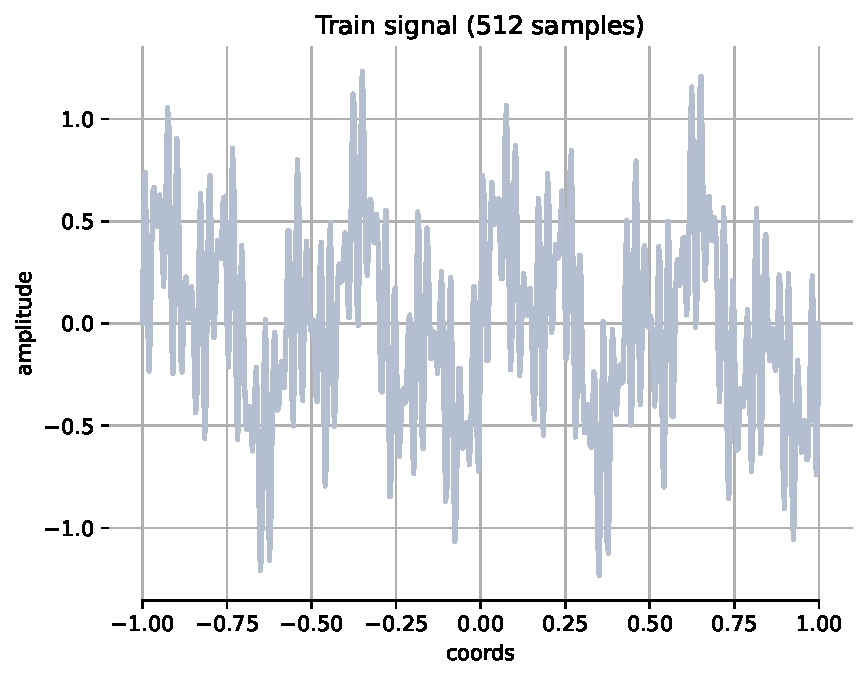
\includegraphics[width=\textwidth]{img/ch4/train_tones512.pdf}
        \caption{Input signal}
        \label{fig:gt-4freqs}
    \end{subfigure}
    \hfill
    \begin{subfigure}[b]{0.32\textwidth}
        \centering
        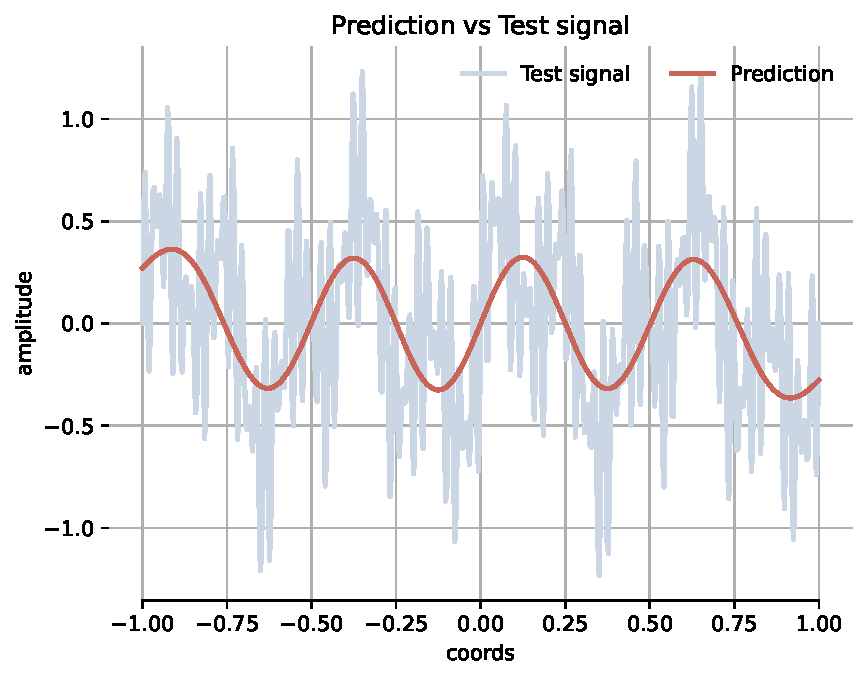
\includegraphics[width=\textwidth]{img/ch4/prediction_w10_smoothed.pdf}
        \caption{Reconstruction}
        \label{fig:rec-naive-w0}
    \end{subfigure}
    \hfill
    \begin{subfigure}[b]{0.32\textwidth}
        \centering
        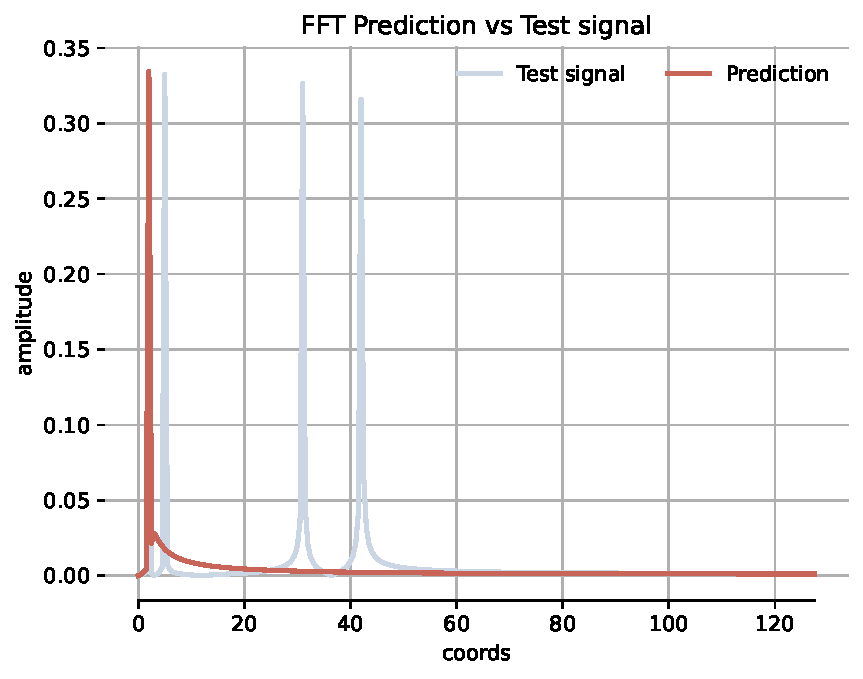
\includegraphics[width=\textwidth]{img/ch4/fft_w10_smoothed.pdf}
        \caption{Frequencies (FFT)}
        \label{fig:fft-smooth-4freqs}
    \end{subfigure}
    \label{f:4freqs-smoothed-reconstruction}
    \caption{Reconstruction of a signal with selected low and high frequencies using a network initialized with very low frequencies.}
\end{figure}


We believe this result is due to the network being initialized with frequencies lower than those present in the signal. Given that the sine function is periodic with a period of $2\pi$, we propose that the hyperparameter $\omega_0$ should always be multiplied by $2\pi$ to better establish a relationship between the initialization of the network's first layer and the range of frequencies represented by each atom in this layer.

Repeating the experiment with $\omega_0 = 10$Hz, that is $10*2\pi$, we observe the expected behavior: the predicted wave in Figure \ref{fig:rec-2pi-w0} approximates the low-frequency portion of the signal. Notice how the FFT plot (Figure \ref{fig:fft-low-4freqs}) matches the peaks at 2 Hz and 5Hz, while the high frequency tones are not learned.

% Since the risk landscape for the SIREN loss has many local minima, is expected that these weights can’t move much further than their initialization, therefore controlling where the weights start should control the range of frequencies one can filter in from the ground truth wave.

\begin{figure}[h!]
    \centering
    \begin{subfigure}[b]{0.38\textwidth}
        \centering
        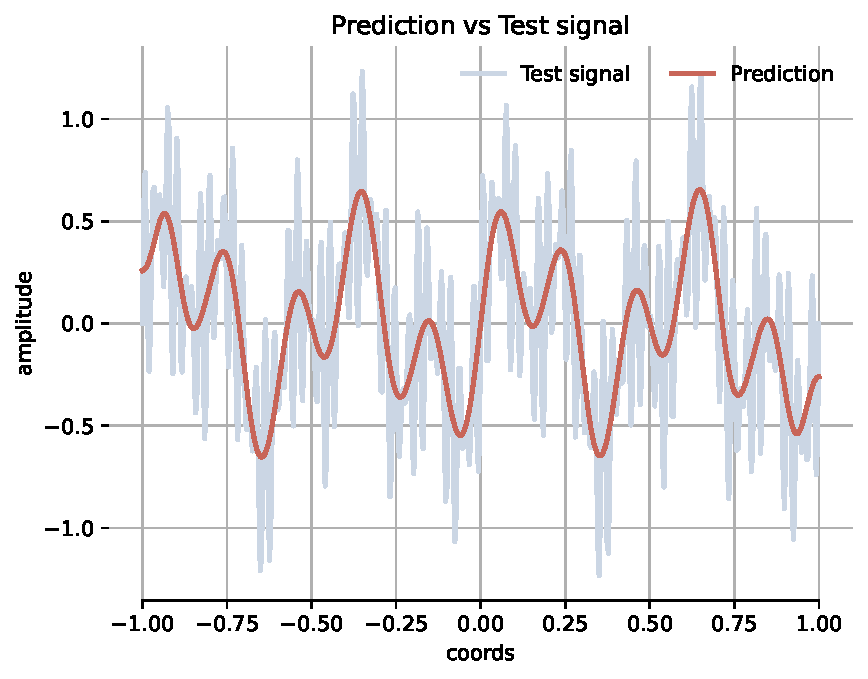
\includegraphics[width=\textwidth]{img/ch4/prediction_w0_2pi.pdf}
        \caption{Reconstruction}
        \label{fig:rec-2pi-w0}
    \end{subfigure}
    % \hfill
    \begin{subfigure}[b]{0.38\textwidth}
        \centering
        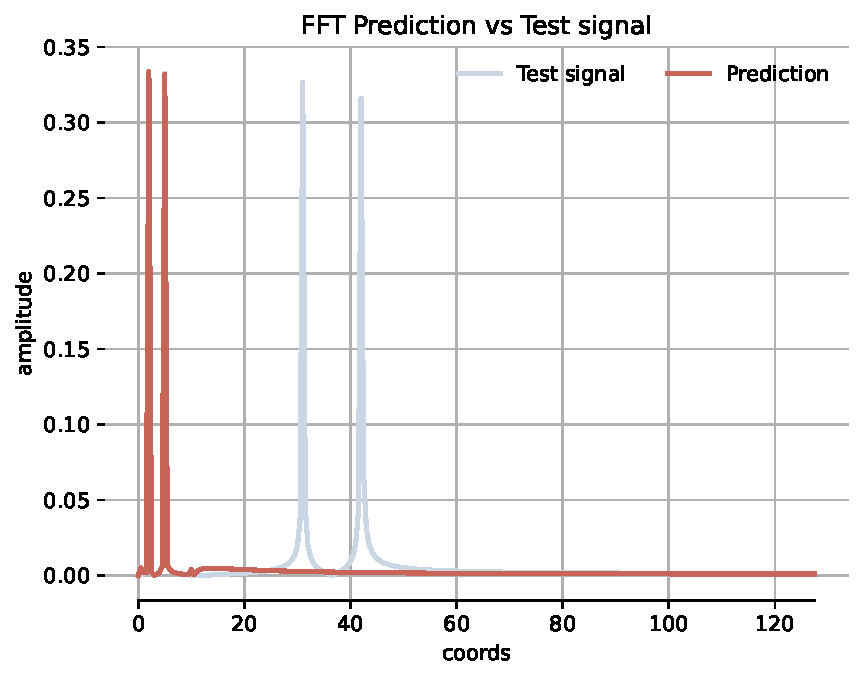
\includegraphics[width=\textwidth]{img/ch4/fft_w0_2pi.pdf}
        \caption{Frequencies (FFT)}
        \label{fig:fft-low-4freqs}
    \end{subfigure}
    \label{f:4freqs-low-reconstruction}
    \caption{Reconstruction of a signal with selected low and high frequencies, where the lower frequencies fall within the initialization range of the network's first layer.}
\end{figure}

Next we change the initialization of the network to frequencies between 25 and 45 Hz. As expected, that also succeeds in predicting the high-frequency tones but fails in capturing the low-frequency ones (Figures \ref{fig:rec-25-45} and \ref{fig:fft-25-45}). Moreover, by initializing the frequencies between 35 and 45 Hz, we are able to isolate the 42 Hz tone (Figures \ref{fig:rec-35-45} and \ref{fig:fft-35-45}).

\begin{figure}[h!]
    \centering
    \begin{subfigure}[b]{0.38\textwidth}
        \centering
        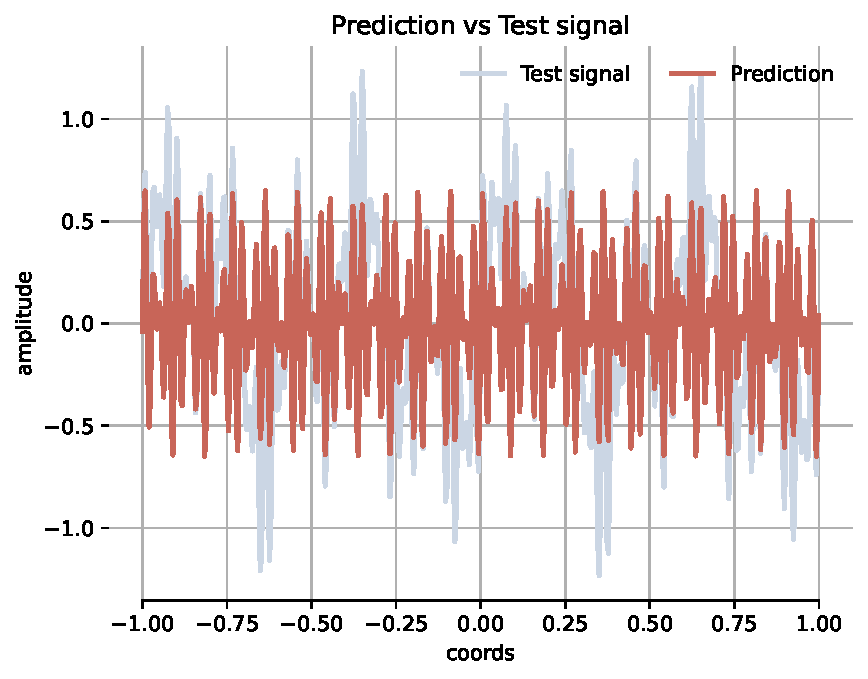
\includegraphics[width=\textwidth]{img/ch4/prediction_w25-45_2pi.pdf}
        \caption{$\omega_0 \in [25, 45]$Hz}
        \label{fig:rec-25-45}
    \end{subfigure}
    % \hfill
    \begin{subfigure}[b]{0.38\textwidth}
        \centering
        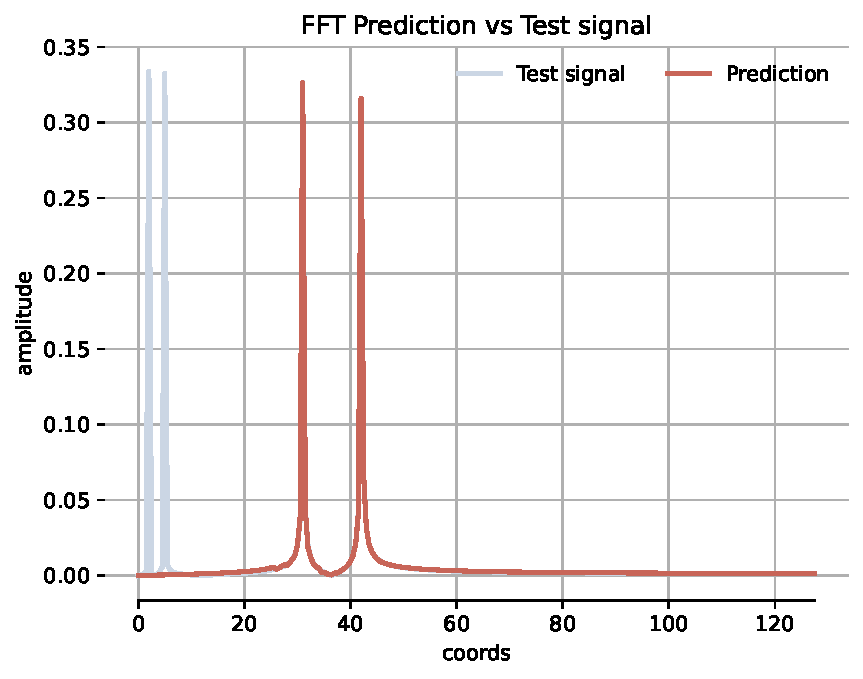
\includegraphics[width=\textwidth]{img/ch4/fft_w25-45.pdf}
        \caption{$\omega_0 \in [25, 45]$Hz}
        \label{fig:fft-25-45}
    \end{subfigure}
    \begin{subfigure}[b]{0.38\textwidth}
        \centering
        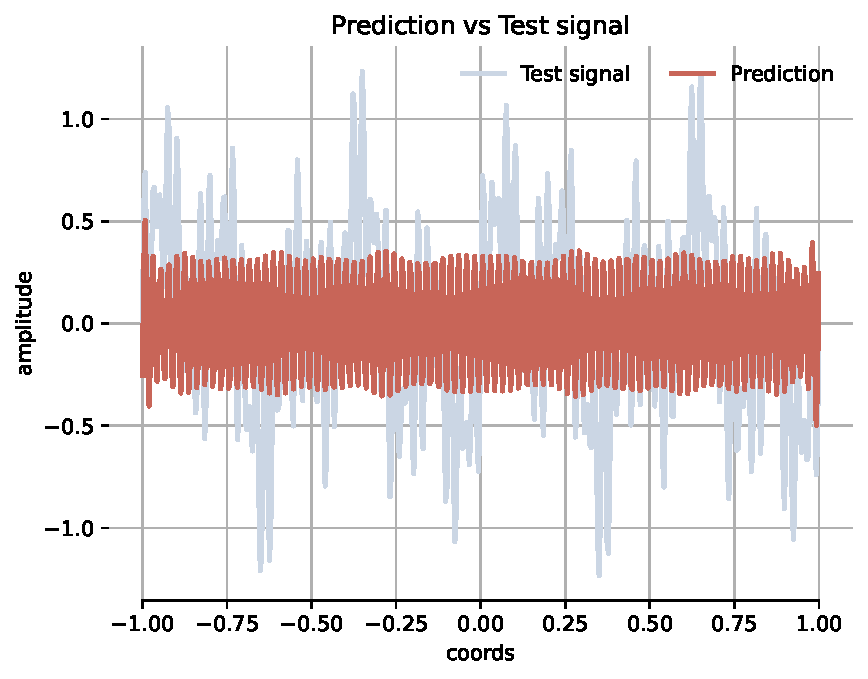
\includegraphics[width=\textwidth]{img/ch4/prediction_w35-45.pdf}
        \caption{$\omega_0 \in [35, 45]$Hz}
        \label{fig:rec-35-45}
    \end{subfigure}
    % \hfill
    \begin{subfigure}[b]{0.38\textwidth}
        \centering
        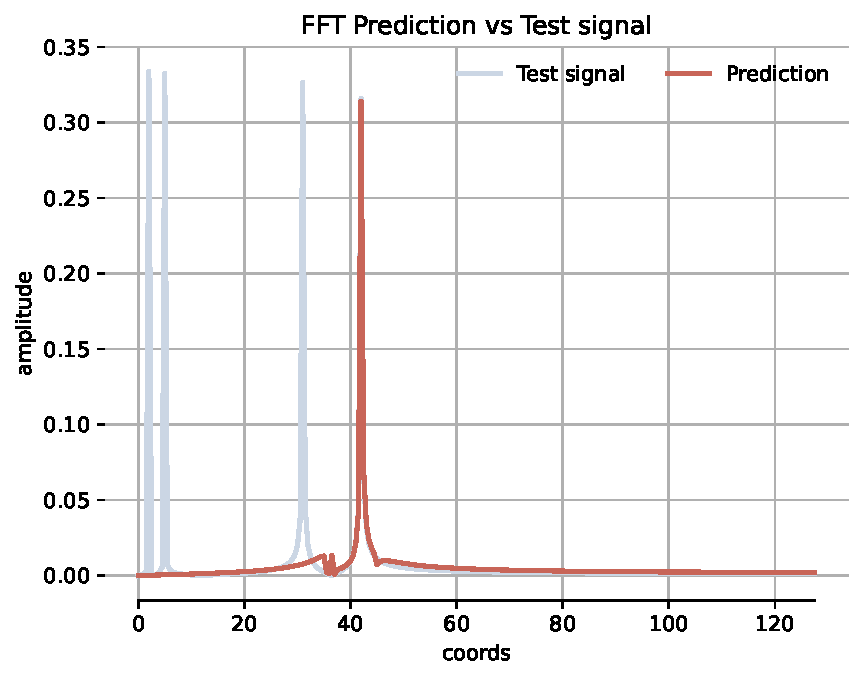
\includegraphics[width=\textwidth]{img/ch4/fft_w35-45.pdf}
        \caption{$\omega_0 \in [35, 45]$Hz}
        \label{fig:fft-35-45}
    \end{subfigure}
    \label{f:high-freqs-reconstruction}
    \caption{Reconstruction of the signal where only the higher frequencies fall within the initialization range of the network’s first layer.}
\end{figure}

Surprisingly, when we use a range of frequencies that encompasses all frequencies present in the input signal, for example $\omega_0 \in [-45, 45]$ Hz, the network does not perfectly fit the signal (Figure \ref{fig:rec-64-full-45}), and a mismatch between the frequencies of the network and of the input signal is evident in the Fast Fourier Transform plot (Figure \ref{fig:fft-64-full-45}). Our hypothesis is that this is due to the network's limited capacity, as it is a shallow network with only 64 neurons per layer. To test this, we repeated the experiment with larger models. Figures \ref{fig:rec-128-full-45} and \ref{fig:fft-128-full-45} show an improvement when the network width is increased to 128 neurons per layer. Note that with 256 neurons, the network can fit the signal perfectly, at least qualitatively, as the reconstructed signal appears to superimpose on the input signal both in the spatial (Figure \ref{fig:rec-256-full-45}) and the spectral (Figure \ref{fig:fft-256-full-45}) domains.

\begin{figure}[h!]
    \centering
    \begin{subfigure}[b]{0.32\textwidth}
        \centering
        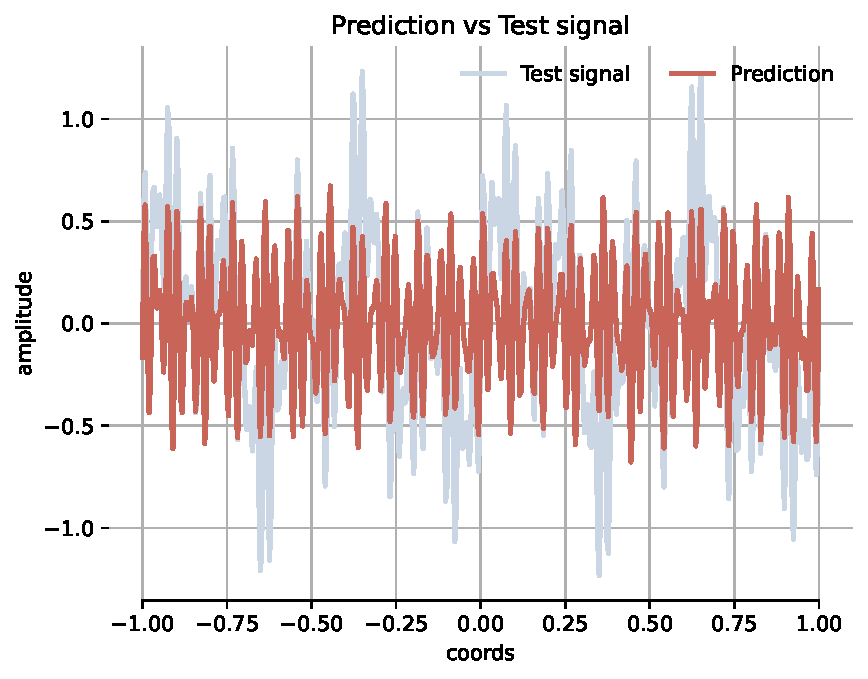
\includegraphics[width=\textwidth]{img/ch4/prediction_w45all_hf64.pdf}
        \caption{64 neurons}
        \label{fig:rec-64-full-45}
    \end{subfigure}
    \hfill
    \begin{subfigure}[b]{0.32\textwidth}
        \centering
        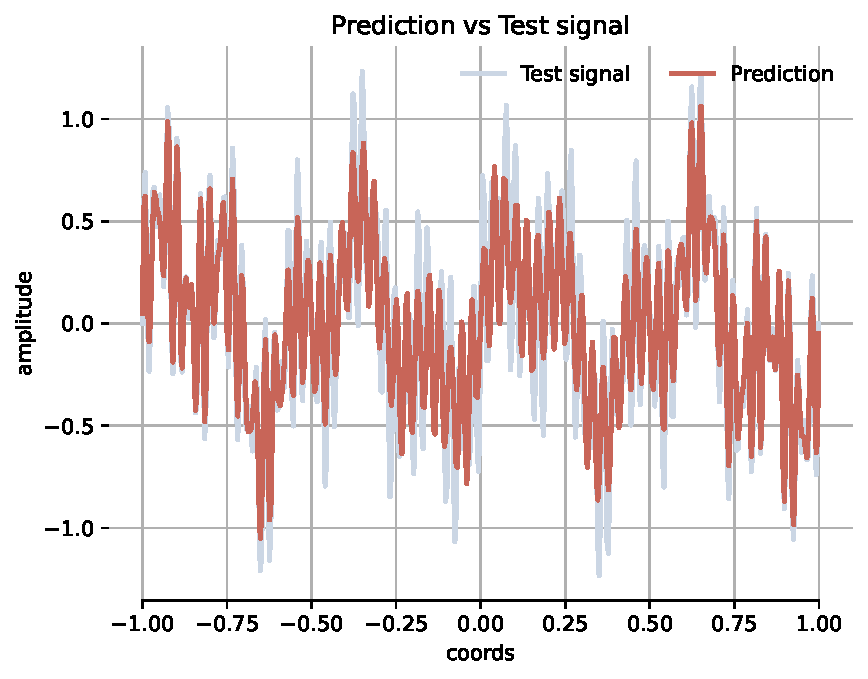
\includegraphics[width=\textwidth]{img/ch4/prediction_w45all_hf128.pdf}
        \caption{128 neurons}
        \label{fig:rec-128-full-45}
    \end{subfigure}
    \begin{subfigure}[b]{0.32\textwidth}
        \centering
        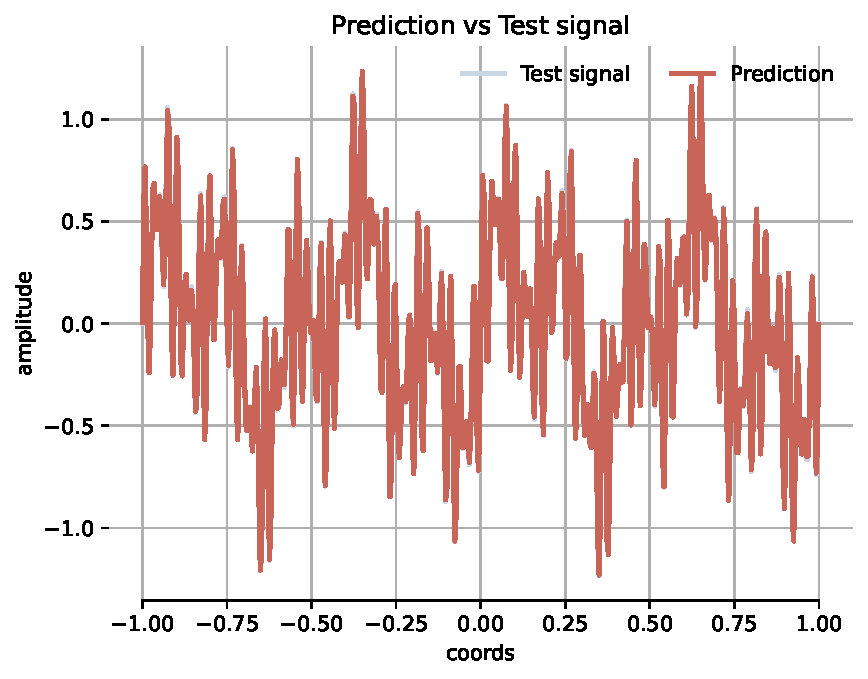
\includegraphics[width=\textwidth]{img/ch4/prediction_w45all_hf256.pdf}
        \caption{256 neurons}
        \label{fig:rec-256-full-45}
    \end{subfigure}
    \begin{subfigure}[b]{0.32\textwidth}
        \centering
        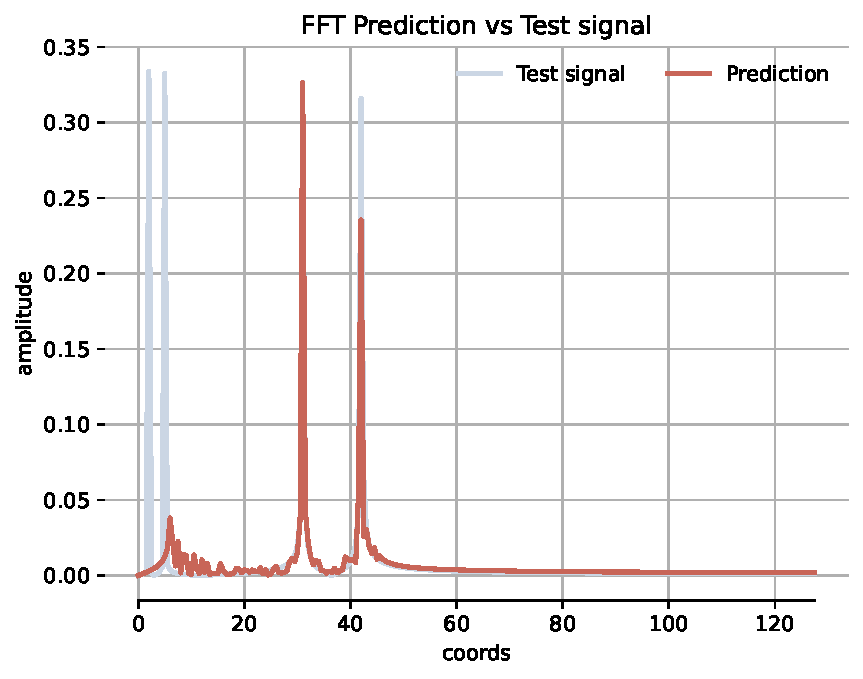
\includegraphics[width=\textwidth]{img/ch4/fft_w45all_hf64.pdf}
        \caption{64 neurons}
        \label{fig:fft-64-full-45}
    \end{subfigure}
    \hfill
    \begin{subfigure}[b]{0.32\textwidth}
        \centering
        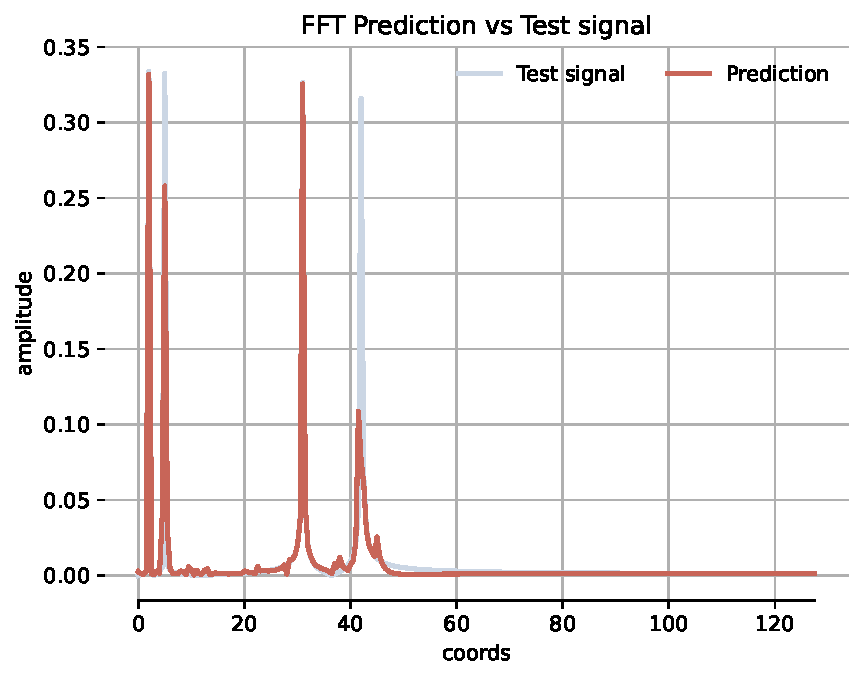
\includegraphics[width=\textwidth]{img/ch4/fft_w45all_hf128.pdf}
        \caption{128 neurons}
        \label{fig:fft-128-full-45}
    \end{subfigure}
    \begin{subfigure}[b]{0.32\textwidth}
        \centering
        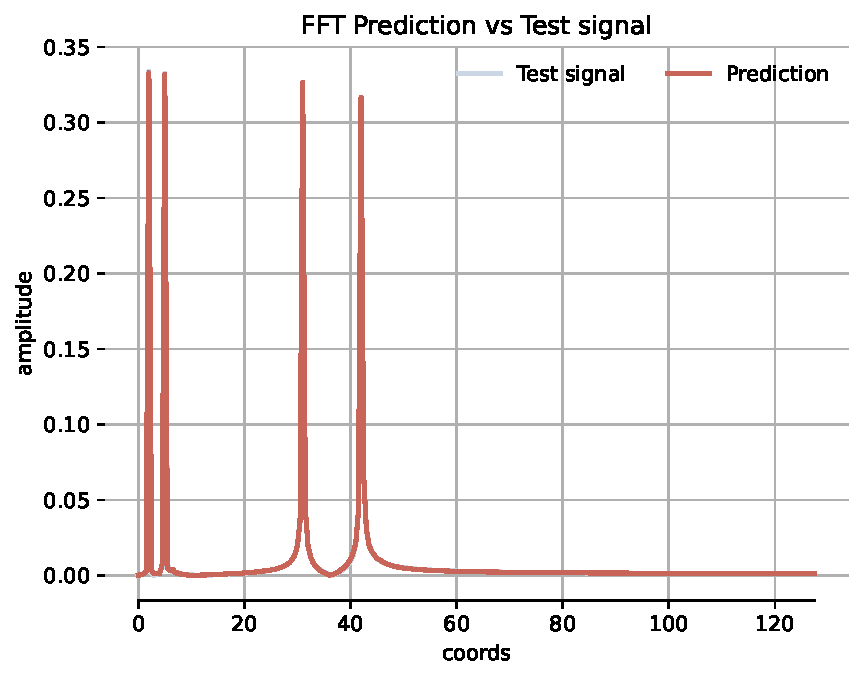
\includegraphics[width=\textwidth]{img/ch4/fft_w45all_hf256.pdf}
        \caption{256 neurons}
        \label{fig:fft-256-full-45}
    \end{subfigure}
    \label{fig:all-freqs-reconstruction}
    \caption{Reconstruction of the signal using networks with different width, all initialized with frequencies in $[-45, 45]$.}
\end{figure}


These experiments validate our hypothesis that a shallow network with only one layer of sinusoidal activation functions can filter a signal by band-limiting its frequency content, providing a spectral filter similar to those in MFN-based architectures. However, when we add a hidden sinusoidal layer to the network, it becomes much more challenging to isolate specific frequencies. Figure \ref{f:w10-1hl-64hf} shows the reconstruction of a sinusoidal network with one hidden layer and 64 neurons per layer, initialized with $\omega_0=10$ Hz. Similar to the experiment with a shallow network of 256 neurons, which was initialized with a broader spectrum of frequencies, the reconstruction seems to perfectly fit the input signal in both the spatial and spectral domains. Figures \ref{fig:4x-freqs-1hl-64hf} and \ref{fig:8x-freqs-1hl-64hf} present two zoomed-in views for a more detailed analysis. In this visualization, the network is evaluated in a grid with 512 samples within a much smaller interval, so most samples were not part of the training data. Notice that the reconstruction is smooth, presenting no spurious noise between the supervised samples.


\begin{figure}[h]
    \centering
    \begin{subfigure}[b]{0.4\textwidth}
        \centering
        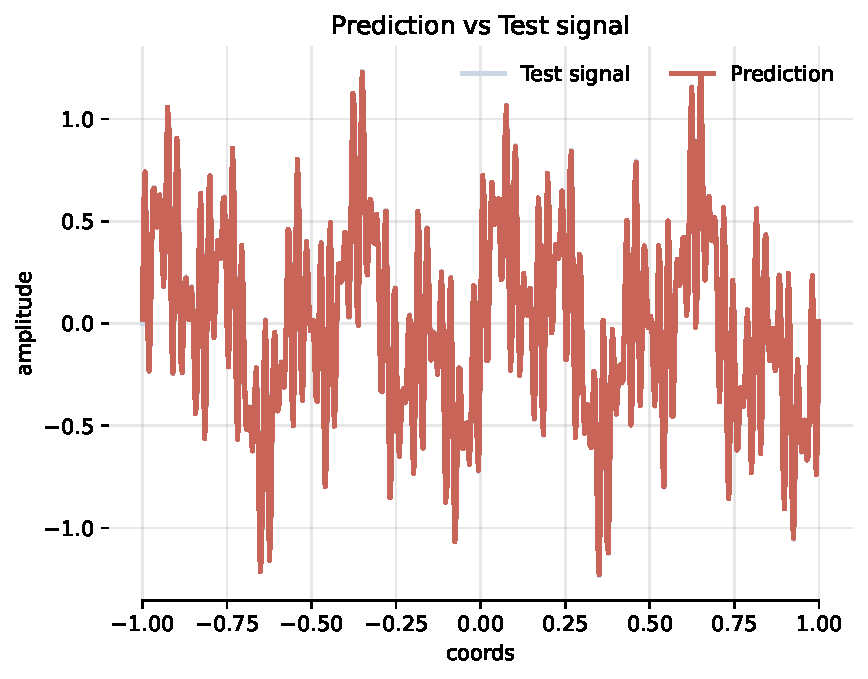
\includegraphics[width=\textwidth]{img/ch4/prediction_1hl_64hf_w10.pdf}
        \caption{Reconstruction}
        \label{fig:rec-freqs-1hl}
    \end{subfigure}
    % \hfill
    \begin{subfigure}[b]{0.4\textwidth}
        \centering
        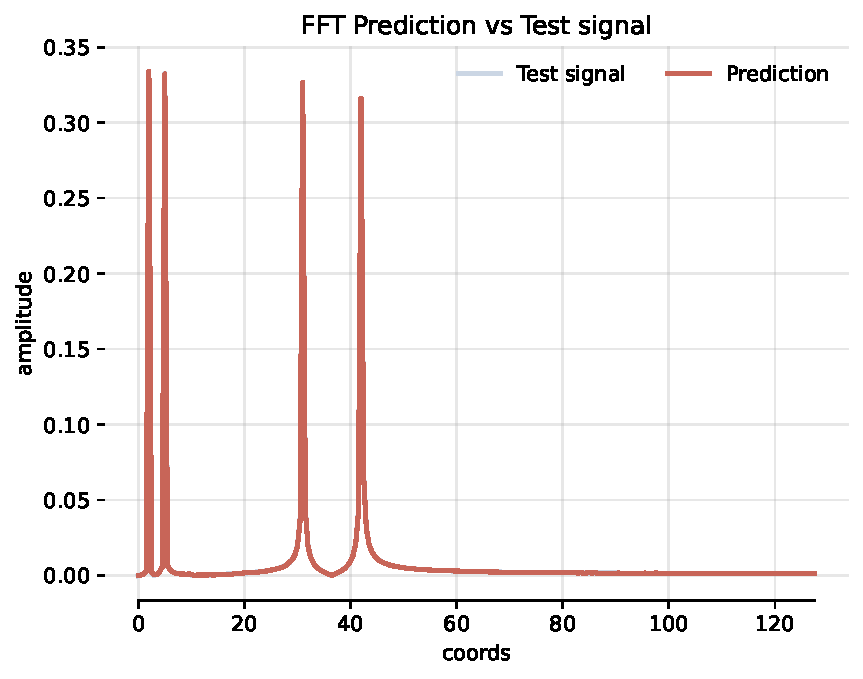
\includegraphics[width=\textwidth]{img/ch4/fft_1hl_64hf_w10.pdf}
        \caption{Frequencies}
        \label{fig:fft-freqs-1hl}
    \end{subfigure}
    
    \begin{subfigure}[b]{0.4\textwidth}
        \centering
        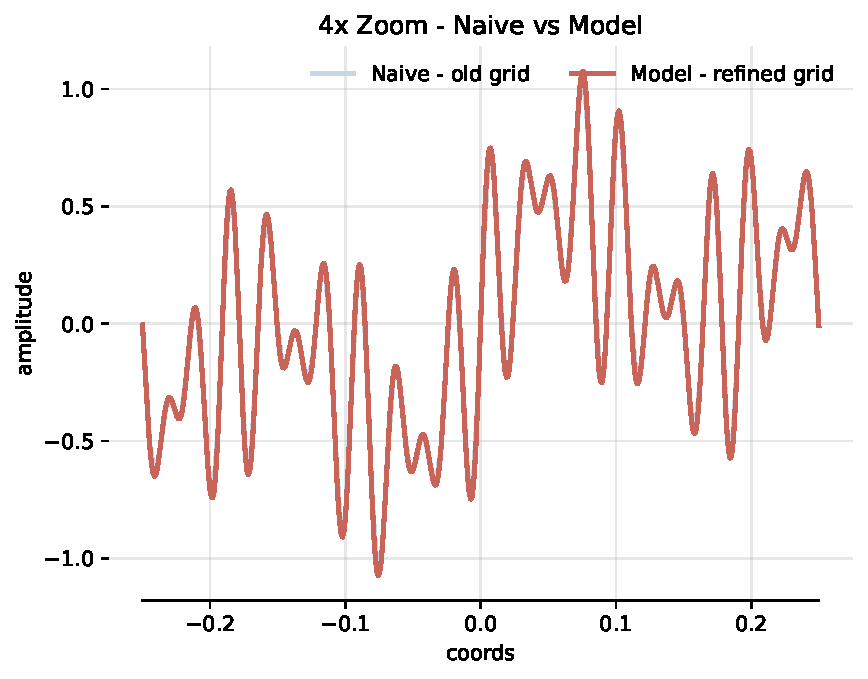
\includegraphics[width=\textwidth]{img/ch4/4x_zoom_1hl_64hf_w10.pdf}
        \caption{Zoom 4x}
        \label{fig:4x-freqs-1hl-64hf}
    \end{subfigure}
    % \hfill
    \begin{subfigure}[b]{0.4\textwidth}
        \centering
        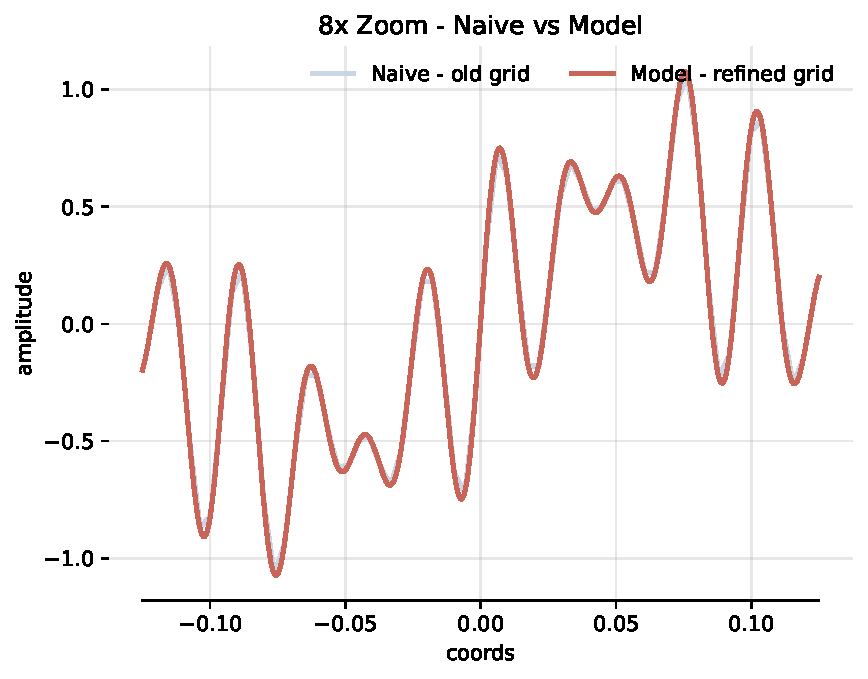
\includegraphics[width=\textwidth]{img/ch4/8x_zoom_1hl_64hf_w10.pdf}
        \caption{Zoom 8x}
        \label{fig:8x-freqs-1hl-64hf}
    \end{subfigure}
    \caption{Reconstruction using 1 hidden layer and 64 neurons per layer.}
    \label{f:w10-1hl-64hf}
\end{figure}

Although the width of the network was kept constant at 64 neurons, adding a single hidden layer significantly increases the size of the model, and thus its capacity, which could explain why it fits the signal better, even though it was initialized with lower frequencies. For instance, a shallow model with 64 neurons per layer has $192$ parameters, while a model with 1 hidden layer and 64 neurons per layer has $4352$ parameters.



To better understand the impact of the hidden layer, we conducted additional experiments, reducing the width of the networks with 1 hidden layer and increasing the width of those without hidden layers. For these experiments, all models were initialized with frequencies in the range $[-10*2\pi, 10*2\pi]$. Figure \ref{fig:rec-1hl-16hf-w10} shows the reconstruction of a model with 1 hidden layer and 16 neurons per layer, with a total of $320$ parameters. Note that this model still captures the high frequencies in the signal, although some noise is visible in its FFT (Figure \ref{fig:fft-1hl-16hf-w10}). However, the model with no hidden layers and 1024 neurons per layer is unable to capture any of the high frequencies (Figures \ref{fig:rec-0hl-1024-w10hf} and \ref{fig:fft-0hl-1024-w10hf}), despite having $3072$ parameters. We conclude that the hidden layer, rather than model size, is primarily responsible for this behavior.

\begin{figure}[h!]
    \centering
    \begin{subfigure}[b]{0.40\textwidth}
        \centering
        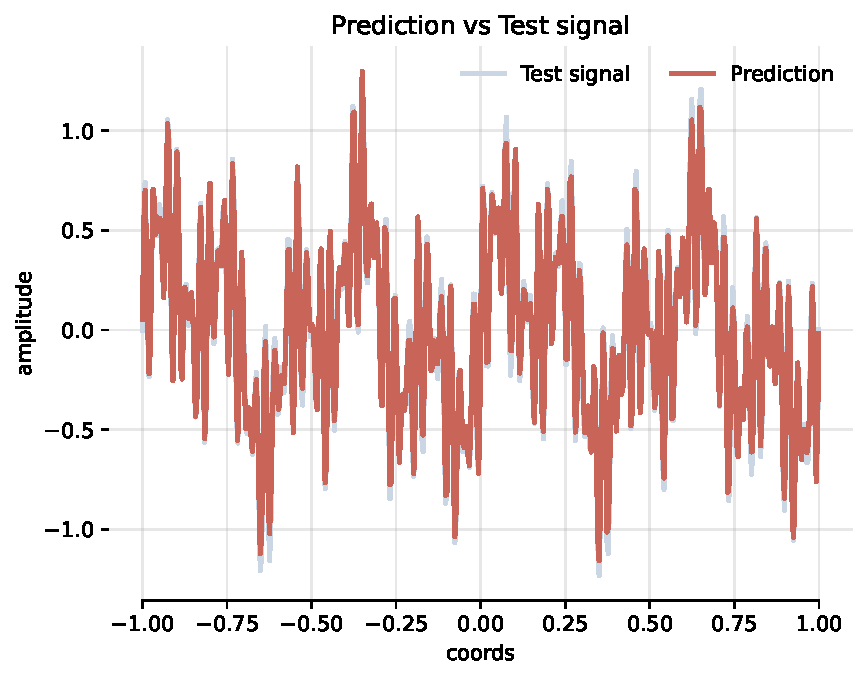
\includegraphics[width=\textwidth]{img/ch4/prediction_1hl_16hf_w10.pdf}
        \caption{1 hidden layer, 16 neurons}
        \label{fig:rec-1hl-16hf-w10}
    \end{subfigure}
    % \hfill
    \begin{subfigure}[b]{0.40\textwidth}
        \centering
        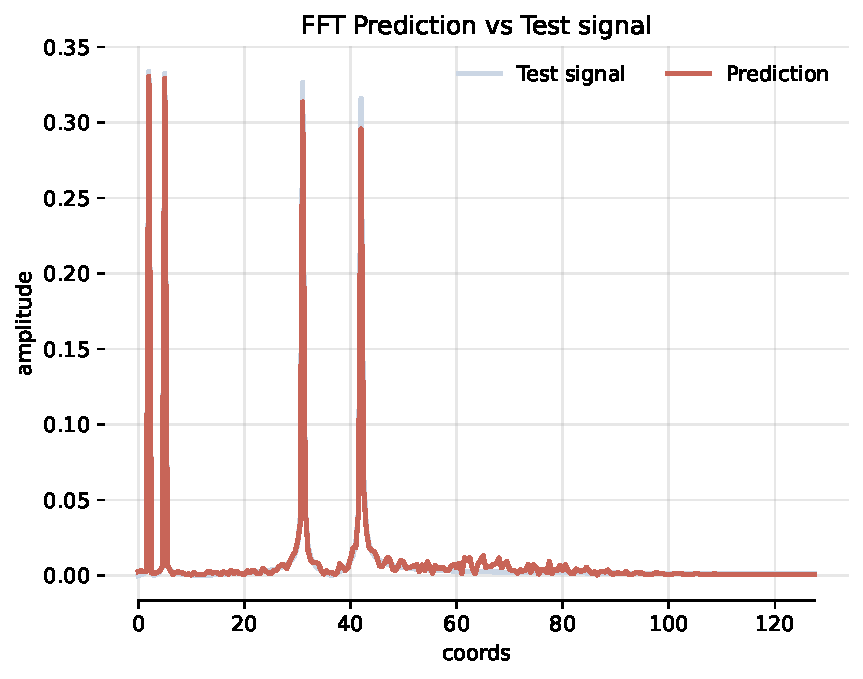
\includegraphics[width=\textwidth]{img/ch4/fft_1hl_16hf_w10.pdf}
        \caption{1 hidden layer, 16 neurons}
        \label{fig:fft-1hl-16hf-w10}
    \end{subfigure}
    
    \begin{subfigure}[b]{0.40\textwidth}
        \centering
        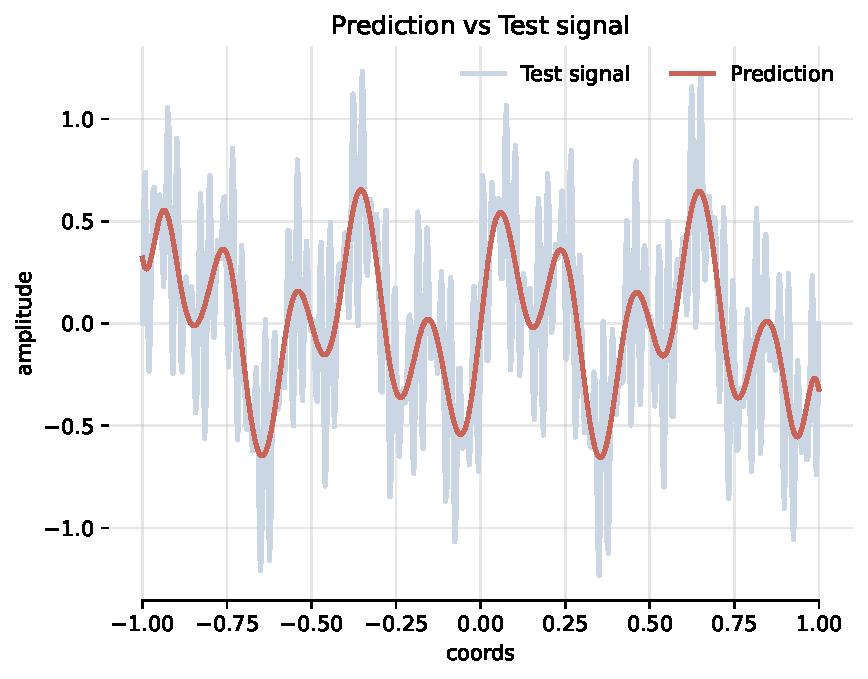
\includegraphics[width=\textwidth]{img/ch4/prediction_0hl_1024hf_w10.pdf}
        \caption{No hidden layers}
        \label{fig:rec-0hl-1024-w10hf}
    \end{subfigure}
    % \hfill
    \begin{subfigure}[b]{0.40\textwidth}
        \centering
        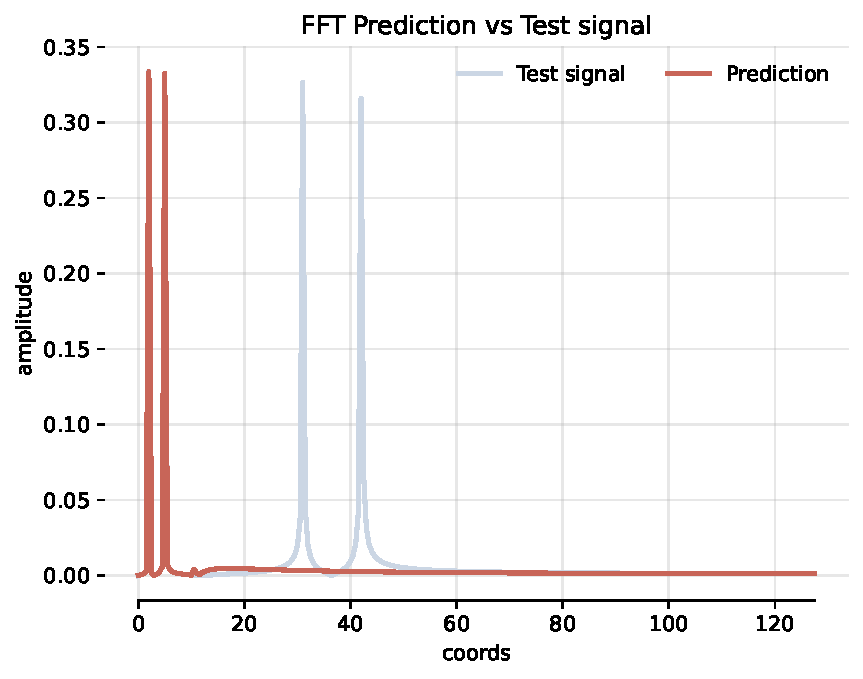
\includegraphics[width=\textwidth]{img/ch4/fft_0hl_1024hf_w10.pdf}
        \caption{No hidden layers}
        \label{fig:fft-0hl-1024-w10hf}
    \end{subfigure}
    \caption{Comparison of a smaller model with a single hidden layer to a larger model without hidden layers.}
    \label{f:hidden-layer-vs-no-hiddel-layer}
\end{figure}

A similar phenomenon is observed when the network is initialized with only the highest frequencies. We ran new experiments with networks initialized with frequencies in the range $[-35*2\pi, -25*2\pi] \cup [25*2\pi, 35*2\pi]$. Figure \ref{fig:rec-1hl-16hf-35w45} shows that a network with 1 hidden layer and 16 neurons per layer can capture the lower frequencies, despite showing some noise in its spectrum (Figure \ref{fig:fft-1hl-16hf-35w45}), while a network with no hidden layers and 1024 neurons per layer fails to capture the lower frequencies (Figures \ref{fig:rec-1hl-1024hf-35w45} and \ref{fig:fft-1hl-1024hf-35w45}).

\begin{figure}
    \centering
    \begin{subfigure}[b]{0.40\textwidth}
        \centering
        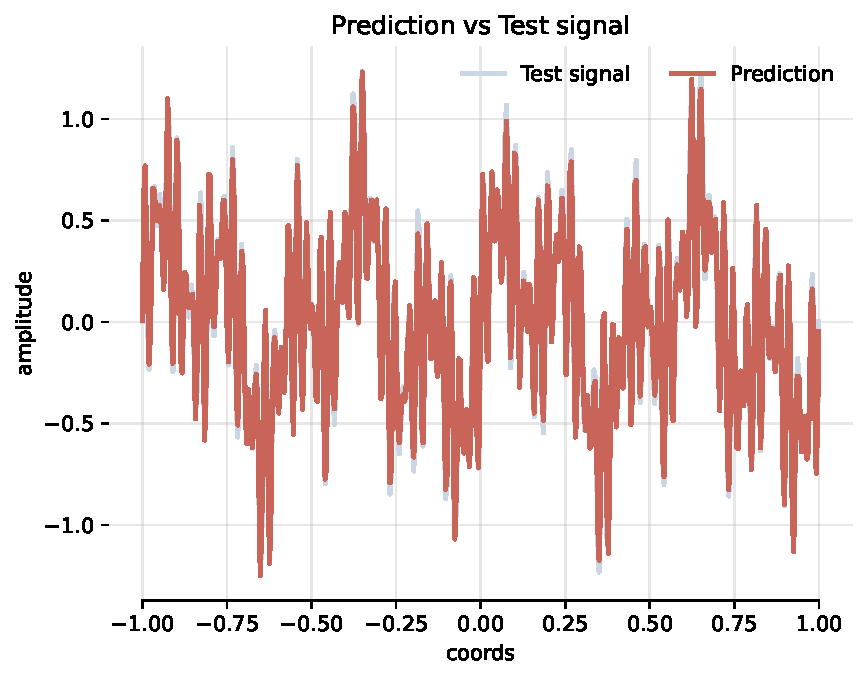
\includegraphics[width=\textwidth]{img/ch4/prediction_1hl_16hf_35w45.pdf}
        \caption{1 hidden layer, 16 neurons}
        \label{fig:rec-1hl-16hf-35w45}
    \end{subfigure}
    % \hfill
    \begin{subfigure}[b]{0.40\textwidth}
        \centering
        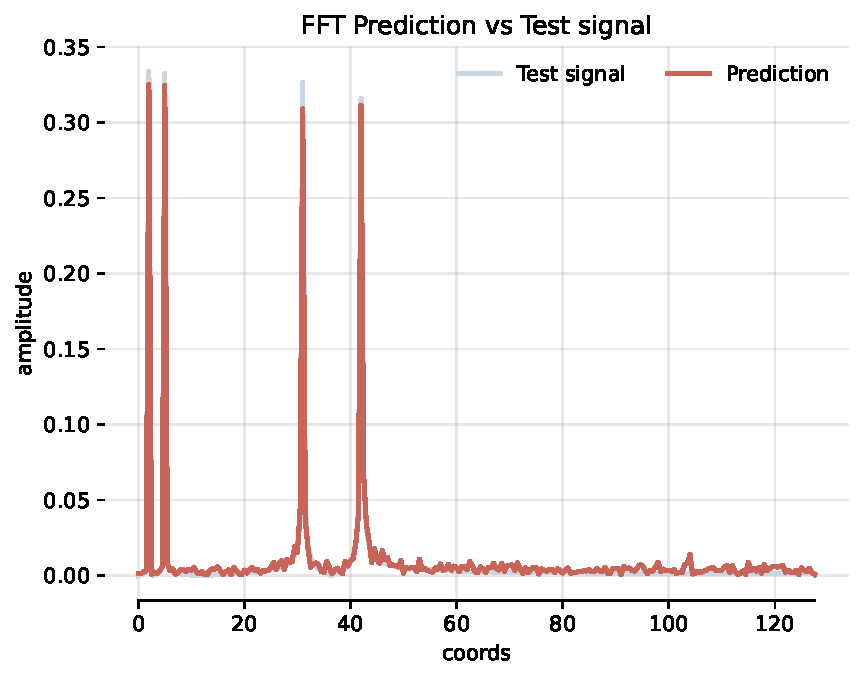
\includegraphics[width=\textwidth]{img/ch4/fft_1hl_16hf_35w45.pdf}
        \caption{1 hidden layer, 16 neurons}
        \label{fig:fft-1hl-16hf-35w45}
    \end{subfigure}
    
    \begin{subfigure}[b]{0.40\textwidth}
        \centering
        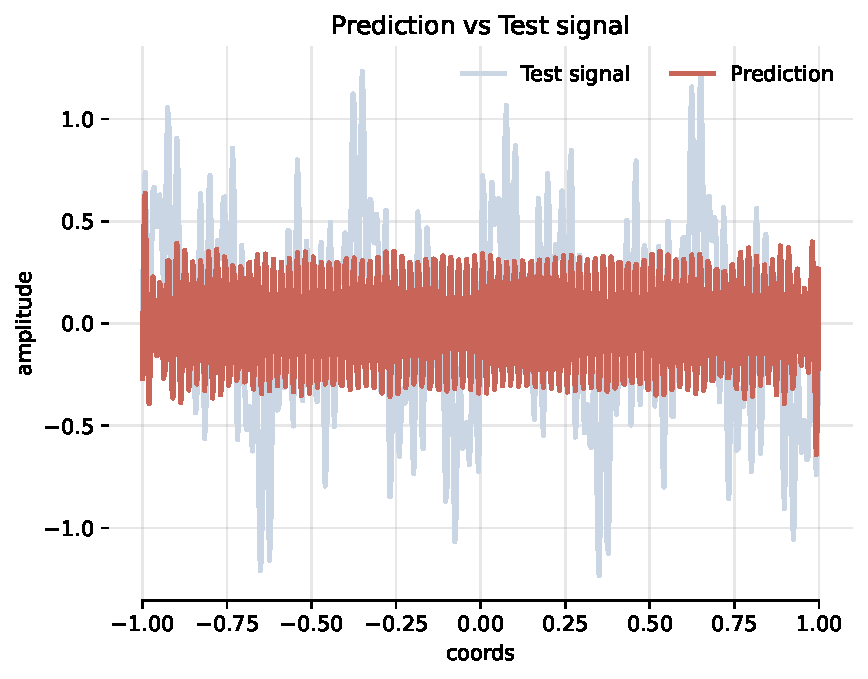
\includegraphics[width=\textwidth]{img/ch4/prediction_1hl_1024hf_35w45.pdf}
        \caption{No hidden layers}
        \label{fig:rec-1hl-1024hf-35w45}
    \end{subfigure}
    % \hfill
    \begin{subfigure}[b]{0.40\textwidth}
        \centering
        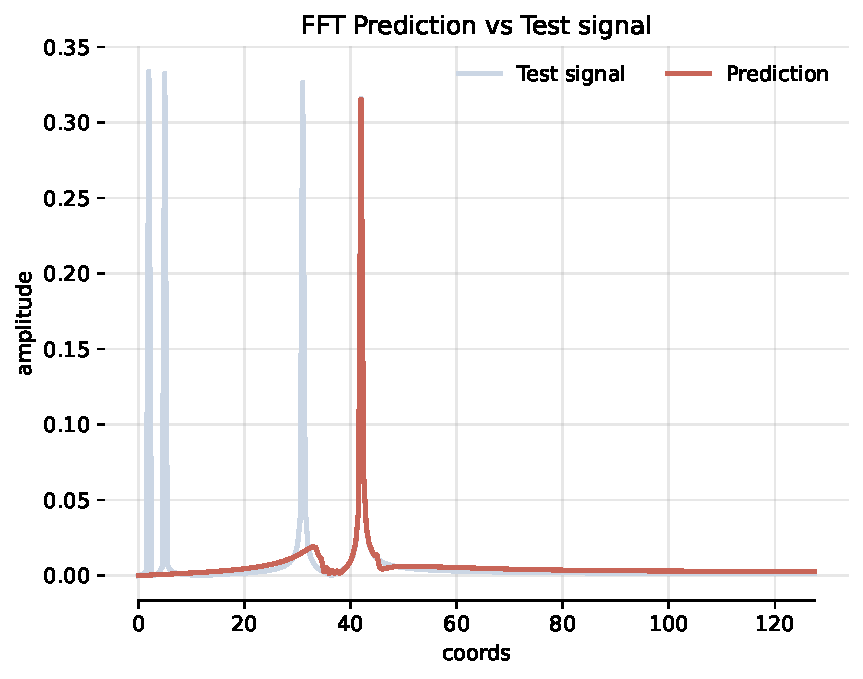
\includegraphics[width=\textwidth]{img/ch4/fft_1hl_1024hf_35w45.pdf}
        \caption{No hidden layers}
        \label{fig:fft-1hl-1024hf-35w45}
    \end{subfigure}
    \caption{Comparison between smaller model with 1 hidden layer and bigger model without hidden layer when models are initialized only with high frequencies.}
    \label{f:hiddenlayer-vs-nohl-high-frequencies}
\end{figure}


We conclude that a sinusoidal neural network with no hidden layers can effectivelly filter and decompose the frequencies of a sinal. However, in general, it not straightforward to decompose the frequencies of a signal using a sinusoidal deep network with at least one hidden layer.

\pagebreak

\subsection{Learning and filtering stochastic signals}

% except in special cases where the signal is simple and the initialization range is very close to the target.

% 4 Multiresolution Sinusoidal Neural Networks

% - Present the experiments in understanding the control of frequencies in a sinusoidal network:
%     - Fitting a signal with few frequencies
%     - Fitting a stochastic signal
%     - Filtering a stochastic signal. Show how the network converges to a filtered version of the signal when initialized with low frequencies. Show the Fourier transform plot.
%     - Diverging by using high frequencies. Show how the network diverges when initialized with very high frequencies.
% - Present the experiments in fitting multiresolution signals
%     - 1D Gaussian Tower
%     - 1D Gaussian Pyramid
%     - show that networks is well behaved between samples
% - Present the MR-Net architecture
%     - Discussion on Filtering, scheduling etc
%     - show the atoms


After experimenting with signals with a few controlled frequencies, we procedurally generated stochastic signals, using a technique known as Perlin Noise \cite{perlin-1985}. This way, we can analyse how a sinusoidal model learns a distribution of frequencies in a broad range. For the following experiments, we sampled 2048 points uniformly in the interval $[-1, 1]$. Thus, the sampling rate is 1/1024. According to the Shannon-Nyquist sampling theorem, we are limited to frequencies up to $512$ Hz. The parameters of the generated Perlin Noise signal are: \red{scale = 10; octaves = 16; persistence = 1.4}.

We start training a shallow sinusoidal network as a sanity check. We expect the network to capture only the lowest frequencies up to the range of frequencies used in its initialization, determined by $\omega_0$. We use a network with 512 hidden neurons per layer and vary the value of $\omega_0$. Figure \ref{f:rec-noise-shallow} shows the reconstruction in spatial and frequency domains for $\omega_0 \in \{8, 64, 128\}$ hz. Note that this time the FFT plot presents a distribution of multiple frequencies up to 512, with a higher amplitude for the lower frenquecies. As expected, the results look like smoothed versions of the signal, as the network captures only the frequencies up to the value of $\omega_0$.

\begin{figure}[h]
    \centering
    \begin{subfigure}[b]{0.32\textwidth}
        \centering
        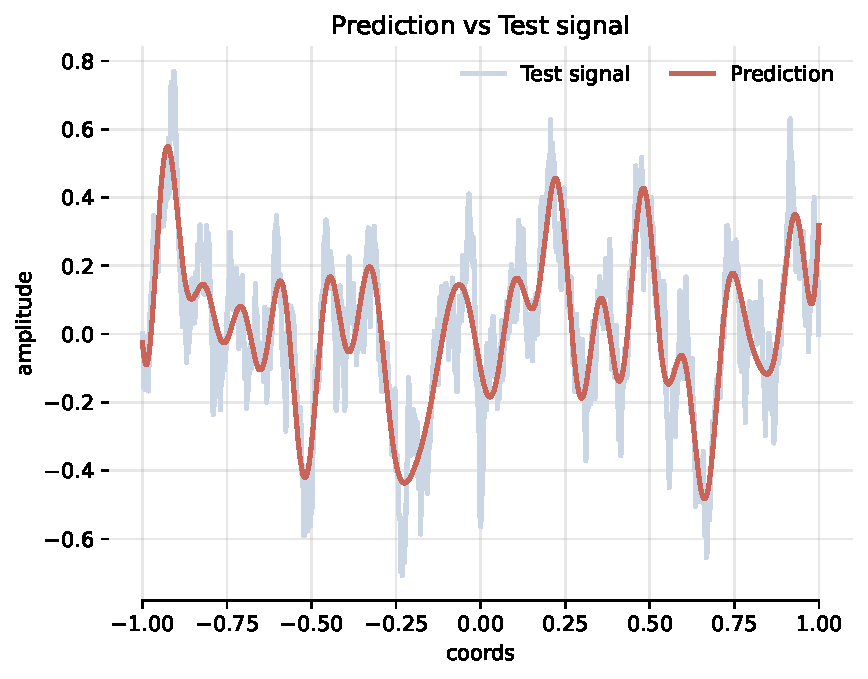
\includegraphics[width=\textwidth]{img/ch4/pred-noise-h0-w8.pdf}
        \caption{$\omega_0=8$}
        \label{fig:rec-noise-shallow-w8}
    \end{subfigure}
    \hfill
    \begin{subfigure}[b]{0.32\textwidth}
        \centering
        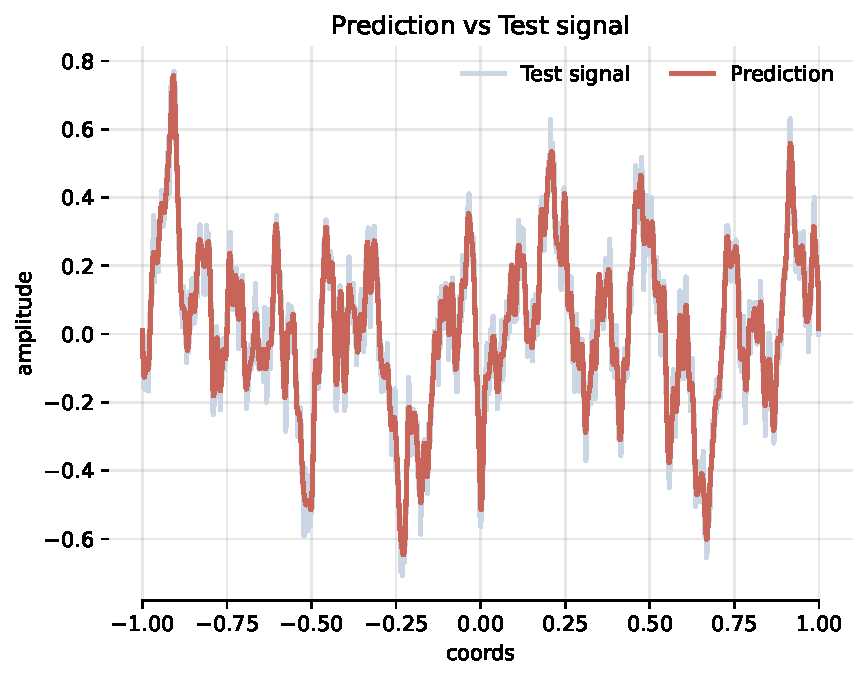
\includegraphics[width=\textwidth]{img/ch4/pred-noise-h0-w64.pdf}
        \caption{$\omega_0=64$}
        \label{fig:rec-noise-shallow-w64}
    \end{subfigure}
    \hfill
    \begin{subfigure}[b]{0.32\textwidth}
        \centering
        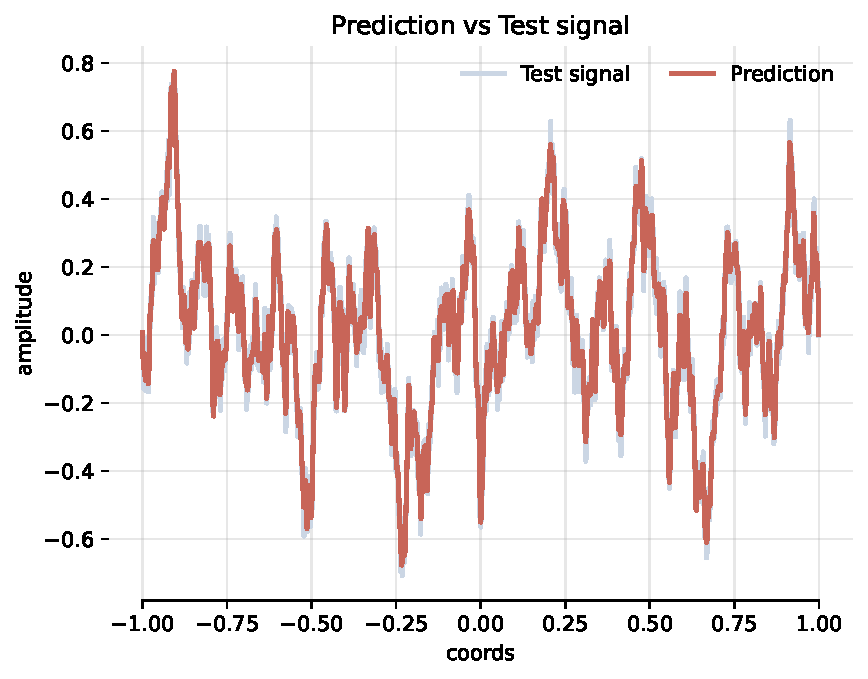
\includegraphics[width=\textwidth]{img/ch4/pred-noise-h0-w128.pdf}
        \caption{$\omega_0=128$}
        \label{fig:rec-noise-shallow-w128}
    \end{subfigure}

    \begin{subfigure}[b]{0.32\textwidth}
        \centering
        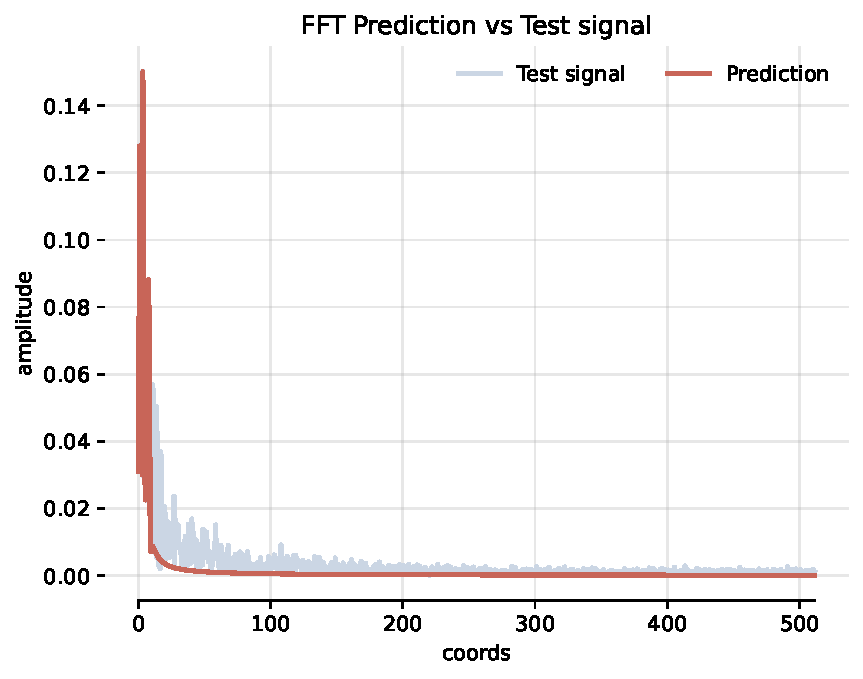
\includegraphics[width=\textwidth]{img/ch4/fft-noise-h0-w8.pdf}
        \caption{$\omega_0=8$}
        \label{fig:fft-noise-shallow-w8}
    \end{subfigure}
    \hfill
    \begin{subfigure}[b]{0.32\textwidth}
        \centering
        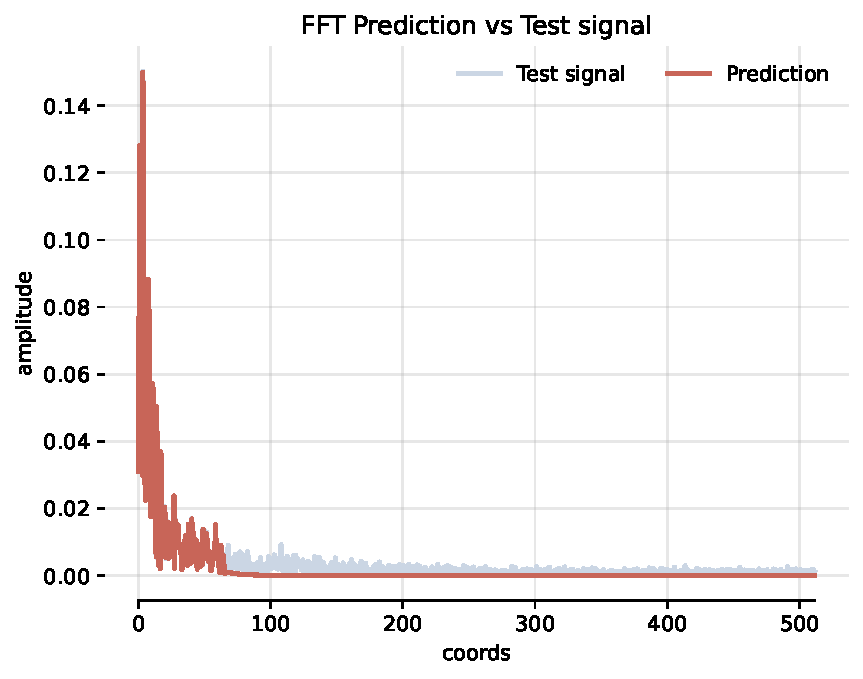
\includegraphics[width=\textwidth]{img/ch4/fft-noise-h0-w64.pdf}
        \caption{$\omega_0=64$}
        \label{fig:fft-noise-shallow-w64}
    \end{subfigure}
    \hfill
    \begin{subfigure}[b]{0.32\textwidth}
        \centering
        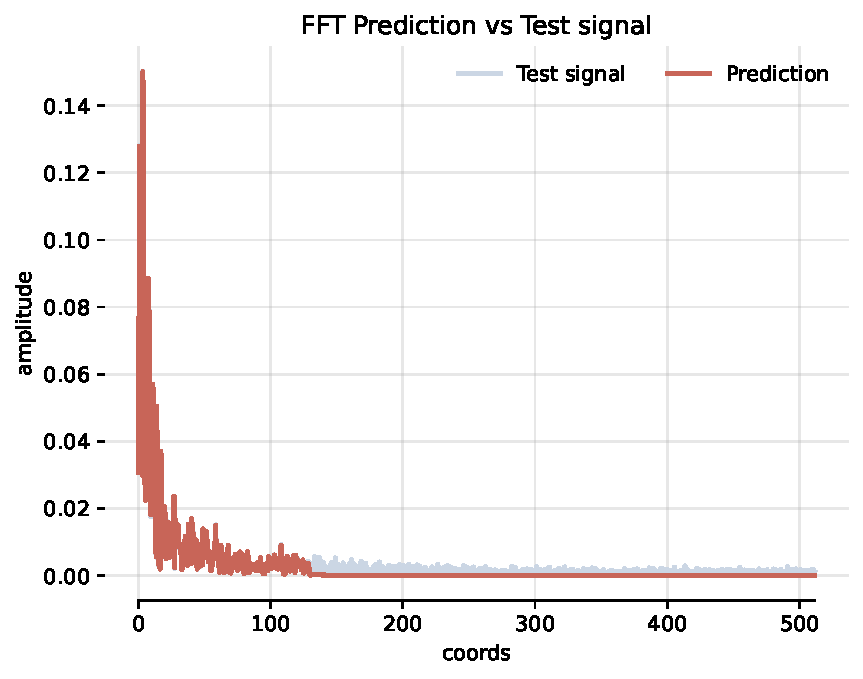
\includegraphics[width=\textwidth]{img/ch4/fft-noise-h0-w128.pdf}
        \caption{$\omega_0=128$}
        \label{fig:fft-noise-shallow-w128}
    \end{subfigure}
    \caption{Reconstruction of a stochastic signal using shallow sinusoidal networks initilized with differente frequency ranges.}
    \label{f:rec-noise-shallow}
\end{figure}

If we keep increasing the value of $\omega_0$ to capture the higher frequencies, we observe a phenomenon similar to what we have seen in Figure \ref{fig:fft-64-full-45}: due to not having enough capacity, the performance of the model decreases in some of the lower frequencies and some noise is produced. Figure \ref{f:rec-noise-shallow-hf512-w256} illustrates this situation.

\begin{figure}[h]
    \centering
    \begin{subfigure}[b]{0.40\textwidth}
        \centering
        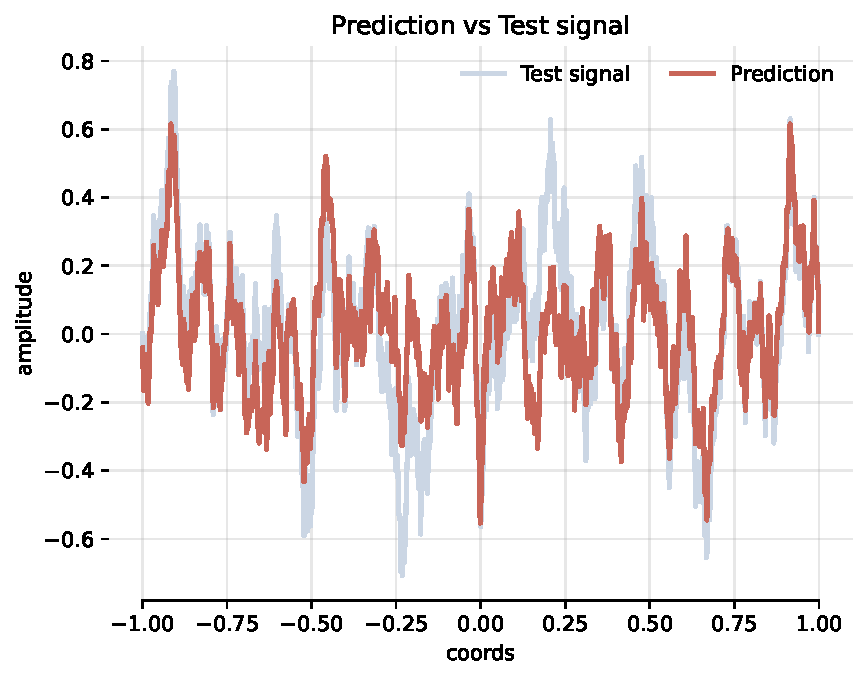
\includegraphics[width=\textwidth]{img/ch4/pred-noise-h0-hf512-w256.pdf}
        \caption{}
        % \label{fig:rec-noise-shallow-hf512-w256}
    \end{subfigure}
    % \hfill
    \begin{subfigure}[b]{0.40\textwidth}
        \centering
        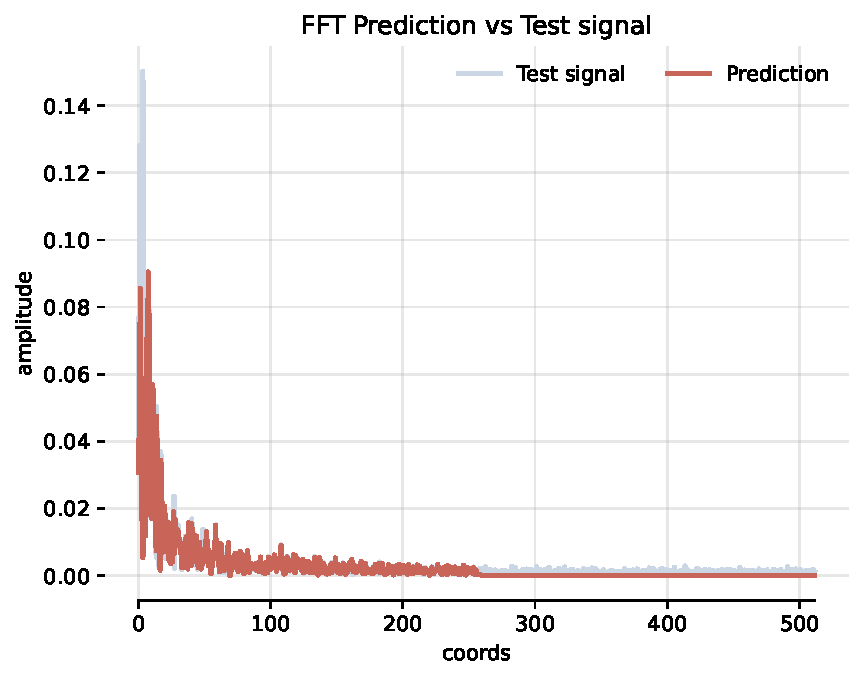
\includegraphics[width=\textwidth]{img/ch4/fft-noise-h0-hf512-w256.pdf}
        \caption{}
        % \label{fig:fft-noise-shallow-hf512-w256}
    \end{subfigure}
    \caption{Reconstruction of signal (A) and frequencies (B) using 512 neurons per layer and $\omega_0=256$}
    \label{f:rec-noise-shallow-hf512-w256}
    % \hfill
    % \begin{subfigure}[b]{0.32\textwidth}
    %     \centering
    %     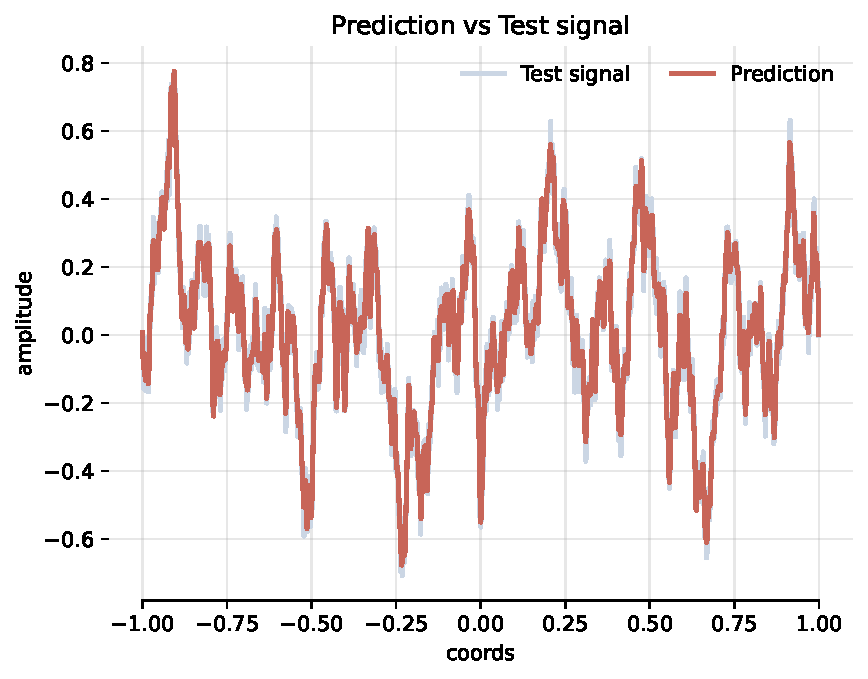
\includegraphics[width=\textwidth]{img/ch4/pred-noise-h0-w128.pdf}
    %     \caption{$\omega_0=128$}
    %     \label{fig:loss-noise-shallow-hf512-w256}
    % \end{subfigure}
\end{figure}

We also observe that the loss function curve becomes bumpy (less smooth) in the experiments with larger frequencies. Figure \ref{f:loss-noise-comparison-hl0-hf512} shows the mean square error per epochs during the training of the network with $\omega_0=64$ and $\omega_0=256$. Based on that, we decreased the learning rate to 0.0001, increased the number of epochs to 400, and ran new experiments. Figure \ref{f:full-noise-hf4096-w512} shows the results of experiments with these new hyperparameters and 4096 neurons per layer; zoomed-in views are provided for better analysis. 


\begin{figure}[h]
    \centering
    \begin{subfigure}[b]{0.45\textwidth}
        \centering
        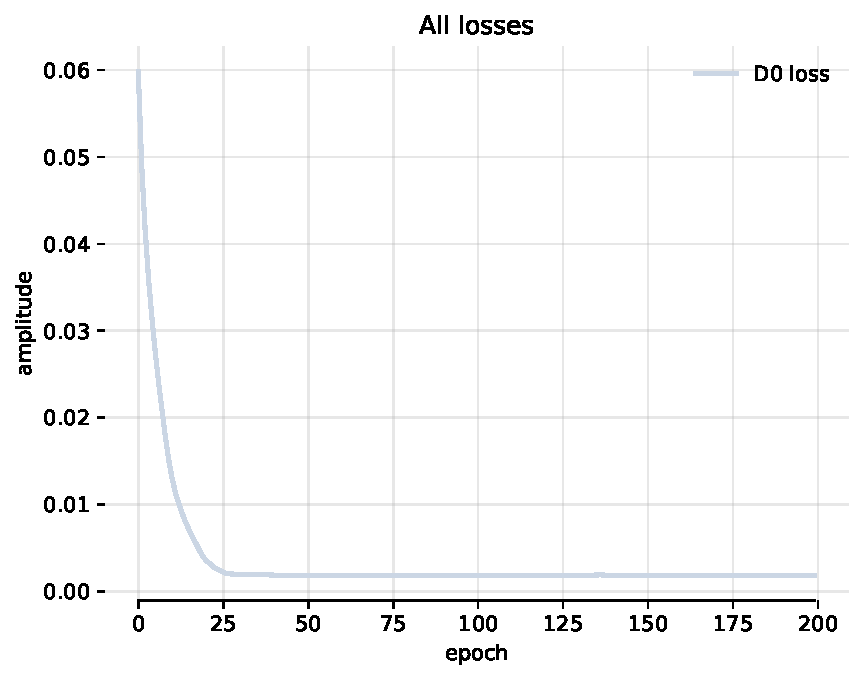
\includegraphics[width=\textwidth]{img/ch4/loss-noise-hl0-hf512-w64.pdf}
        \caption{$\omega_0=64$}
        \label{fig:loss-hf512-w64}
    \end{subfigure}
    \begin{subfigure}[b]{0.45\textwidth}
        \centering
        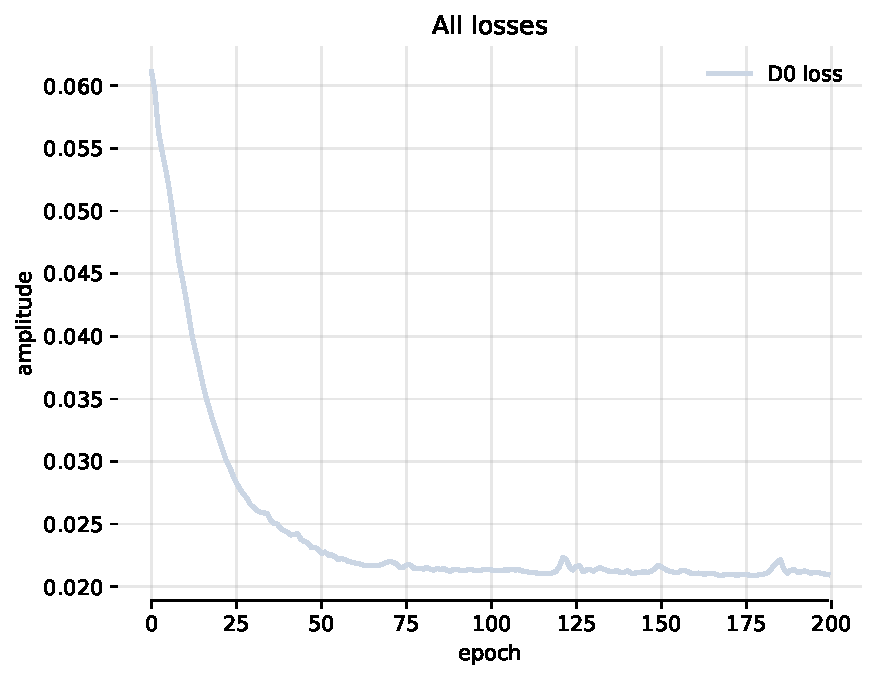
\includegraphics[width=\textwidth]{img/ch4/loss-noise-hl0-hf512-w256.pdf}
        \caption{$\omega_0=256$}
        \label{fig:loss-hf512-w256}
    \end{subfigure}
    \caption{Mean squared error per epoch.}
    \label{f:loss-noise-comparison-hl0-hf512}
\end{figure}


\begin{figure}[h]
    \centering
    \begin{subfigure}[b]{0.32\textwidth}
        \centering
        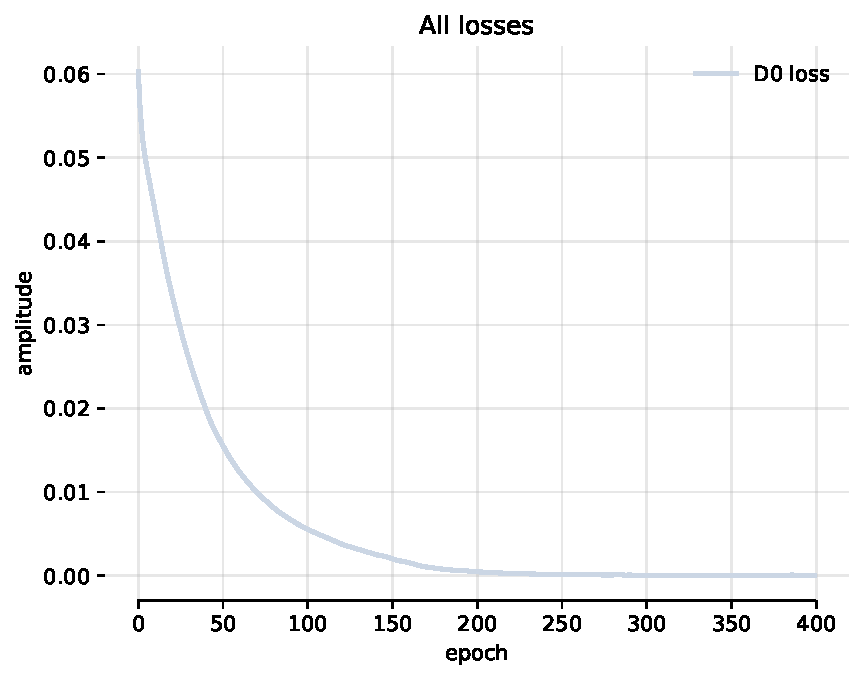
\includegraphics[width=\textwidth]{img/ch4/loss-noise-hf4096-w512.pdf}
        \caption{Loss}
    \end{subfigure}
    \begin{subfigure}[b]{0.32\textwidth}
        \centering
        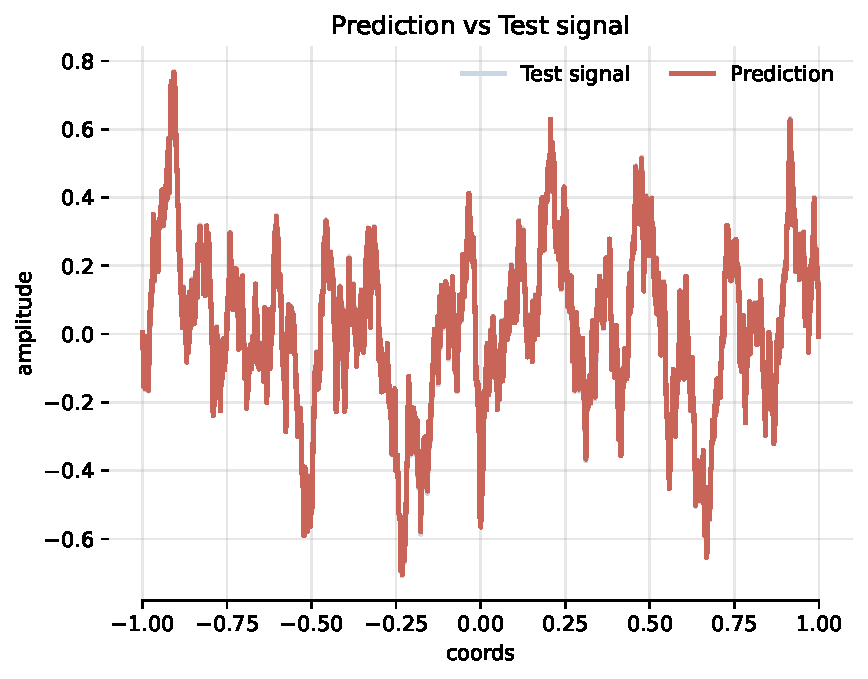
\includegraphics[width=\textwidth]{img/ch4/pred-noise-hf4096-w512.pdf}
        \caption{Reconstruction}
    \end{subfigure}
    \begin{subfigure}[b]{0.32\textwidth}
        \centering
        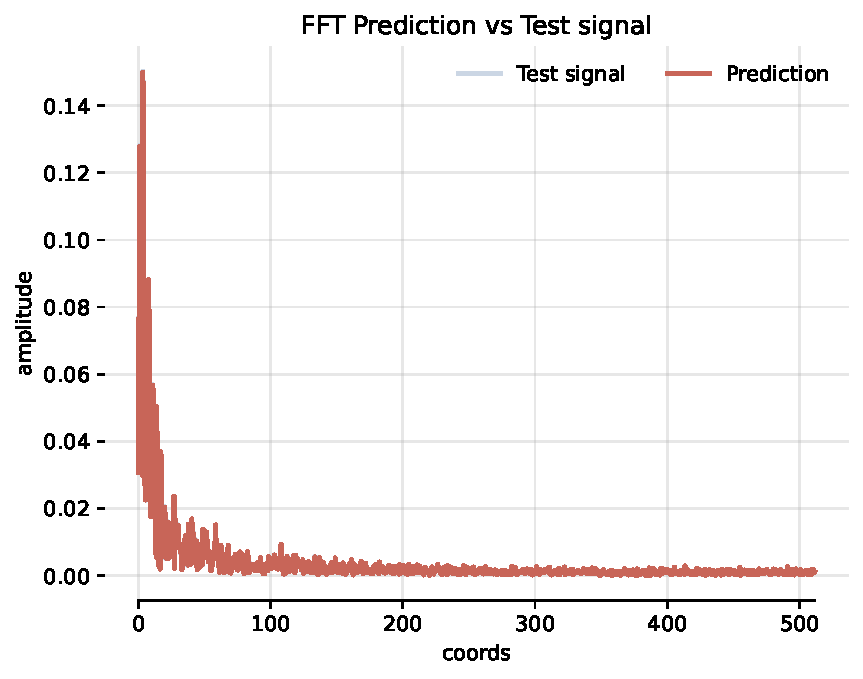
\includegraphics[width=\textwidth]{img/ch4/fft-noise-hf4096-w512.pdf}
        \caption{Frequencies}
    \end{subfigure}

    \begin{subfigure}[b]{0.32\textwidth}
        \centering
        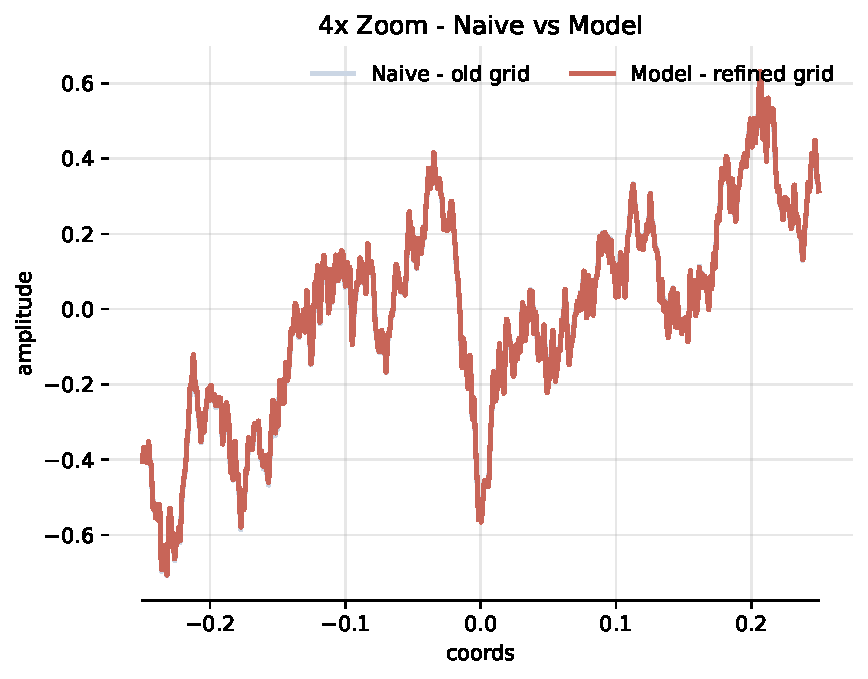
\includegraphics[width=\textwidth]{img/ch4/noise-4x-hf4096-w512.pdf}
        \caption{4x zoom}
    \end{subfigure}
    \begin{subfigure}[b]{0.32\textwidth}
        \centering
        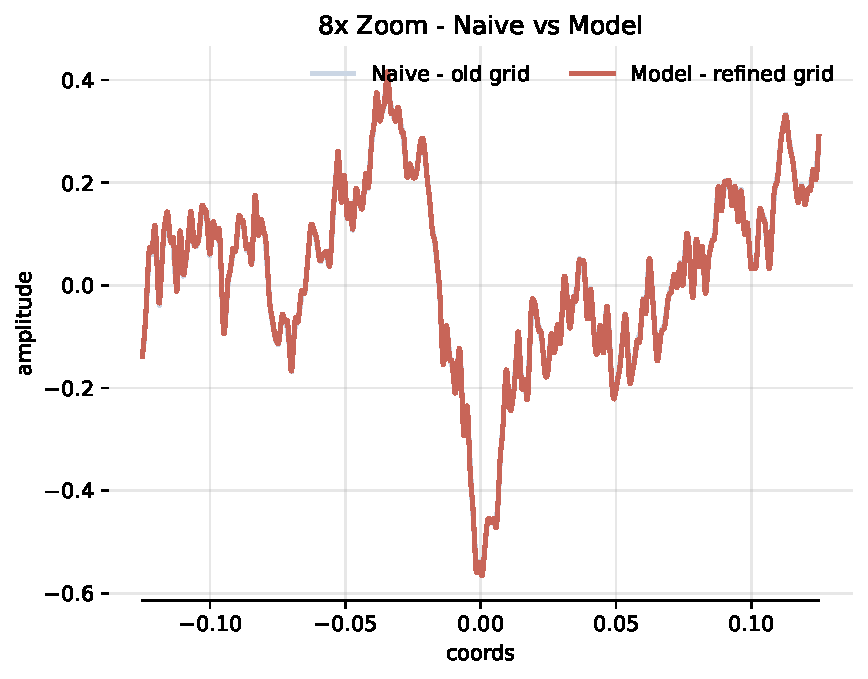
\includegraphics[width=\textwidth]{img/ch4/noise-8x-hf4096-w512.pdf}
        \caption{8x zoom}
    \end{subfigure}
    \begin{subfigure}[b]{0.32\textwidth}
        \centering
        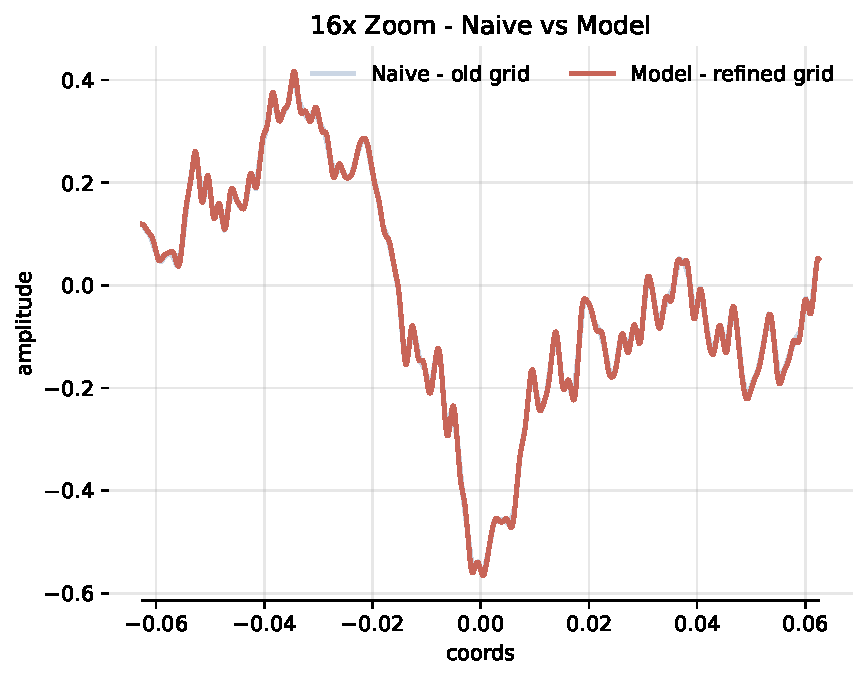
\includegraphics[width=\textwidth]{img/ch4/noise-16x-hf4096-w512.pdf}
        \caption{16x zoom}
    \end{subfigure}
    \caption{Reconstruction results using a shallow network with 4096 neurons per layer and $\omega_0=512$}
    \label{f:full-noise-hf4096-w512}
\end{figure}


In the next experiments, we have employed sinusoidal neural networks with one hidden layer. The main question we want to investigate is: can we learn bounded frequencies using smaller (but deeper) networks? The answer is "yes", but we should be careful (make it the right way).

First, we must notice that introducing a hidden layer greatly increases the capacity of the network on generating higher frequencies. Figure \ref{rec-1hl-32hf-8hz} shows the reconstruction of the same Perlin noise used the previous experiments, but using a neural network with 1 hidden layer and 32 neurons per layer, initialized with $\omega_0=8$Hz. As in the first experiments with shallow networks, we have trained trained for 200 epochs with a learning rate of 0.001. 


\begin{figure}[h]
    \centering
    \begin{subfigure}[b]{0.32\textwidth}
        \centering
        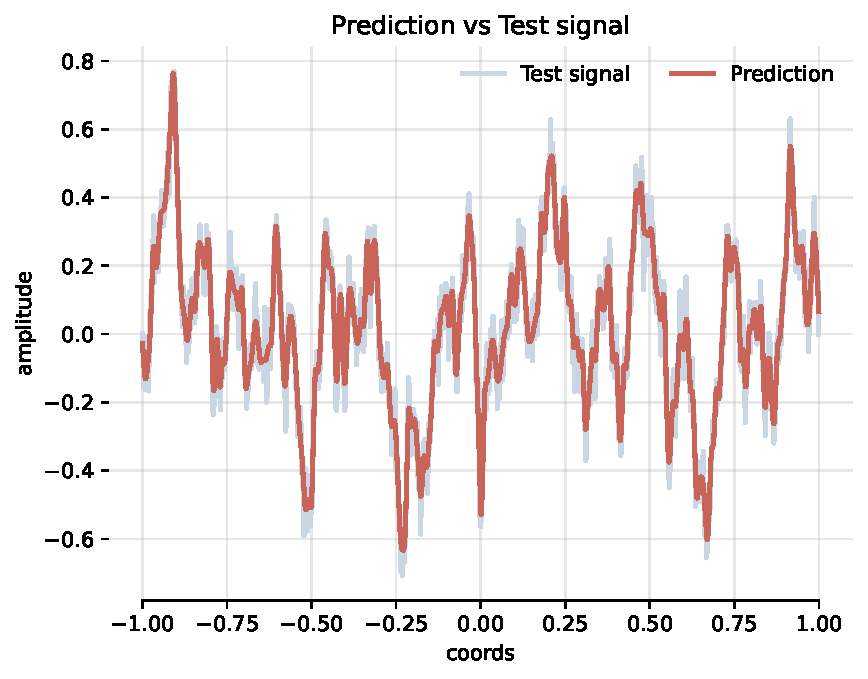
\includegraphics[width=\textwidth]{img/ch4/pred-noise-1hl-32hf-w8.pdf}
        \caption{}
        \label{fig:pred-noise-1hl-32hf-w8}
    \end{subfigure}
    \begin{subfigure}[b]{0.32\textwidth}
        \centering
        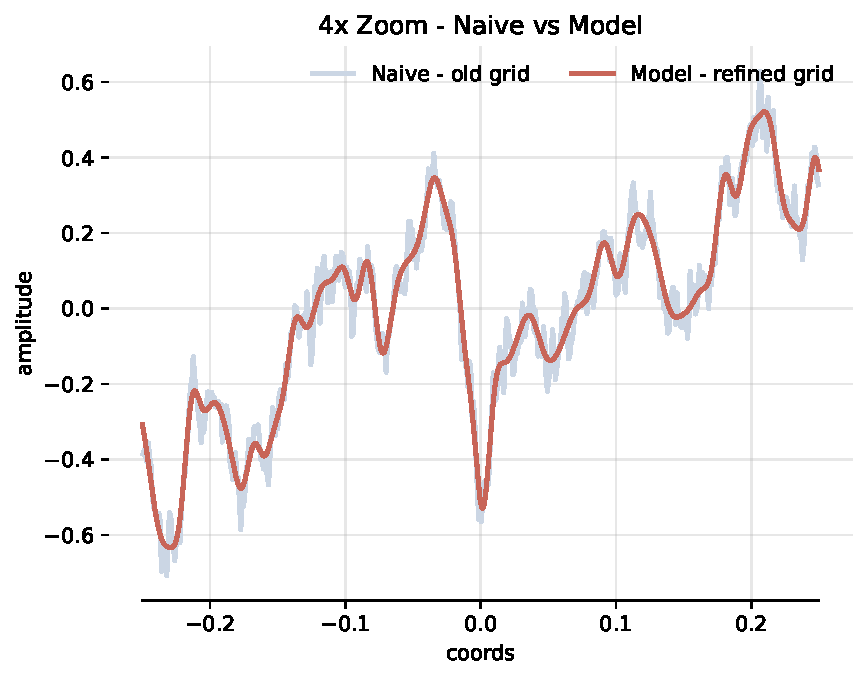
\includegraphics[width=\textwidth]{img/ch4/4x-zoom-noise-1hl-32hf-w8.pdf}
        \caption{}
        \label{fig:4x-zoom-noise-1hl-32hf-w8}
    \end{subfigure}
    \begin{subfigure}[b]{0.32\textwidth}
        \centering
        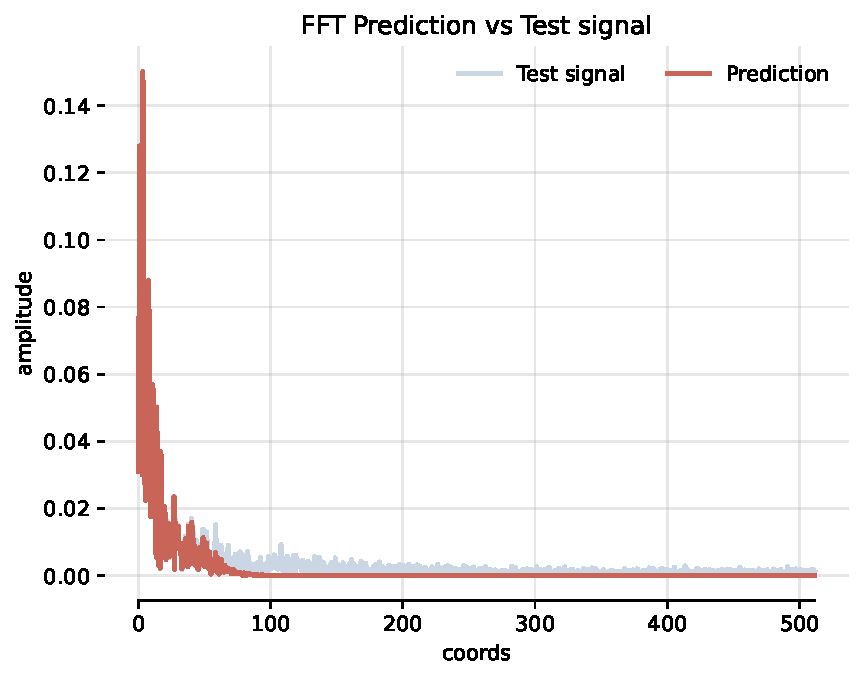
\includegraphics[width=\textwidth]{img/ch4/fft-noise-1hl-32hf-w8.pdf}
        \caption{}
        \label{fig:fft-noise-1hl-32hf-w8}
    \end{subfigure}
    \caption{Smoothed reconstruction with 1 hidden layer}
    \label{f:rec-1hl-32hf-8hz}
\end{figure}

The result in Figure \ref{fig:pred-noise-1hl-32hf-w8} looks like a smoothed version of the input signal, as expected. It can be better seen in the zoomed-in view (Figure \ref{fig:4x-freqs-1hl-64hf}). However, the Fast Fourier Transform (Figure \ref{fig:fft-noise-1hl-32hf-w8}) displays frequecies much higher than 8 Hz, in contrast with the experiment with larger but shallow network Figures (\ref{fig:rec-noise-shallow-w8} and \ref{fig:fft-noise-shallow-w8}). Notice how the Fast Fourier Transform of the reconstructed signal matches that of the original signal up to a value around 30 Hz, then it fails to capture the exact contribution of frequencies in a range that goes until around 100hz, and finally it does not exhibit contributions of frequencies higher than 100 hz.


Decreasing the number of neurons per layer slightly decreases the hightest frequencies learned by the network while increasing its width, also increases the highest frequencies captured as illustrated in Figure \ref{f:comparison-16-32-64-hf}. This is directly read from the FFT plots (Figures \ref{fig:fft-noise-1hl-16hf-w8}, \ref{fig:fft-noise-1hl-32hf-w8} and \ref{fig:fft-noise-1hl-64hf-w8}) but can also be perceived by the most refined details in the spatial reconstruction of the signal (Figures \ref{fig:4x-zoom-noise-1hl-16hf-w8}, \ref{fig:comp-4x-zoom-noise-1hl-32hf-w8} and \ref{fig:4x-zoom-pred-noise-1hl-64hf-w8}).



\begin{figure}[h]
    \centering
    \begin{subfigure}[b]{0.32\textwidth}
        \centering
        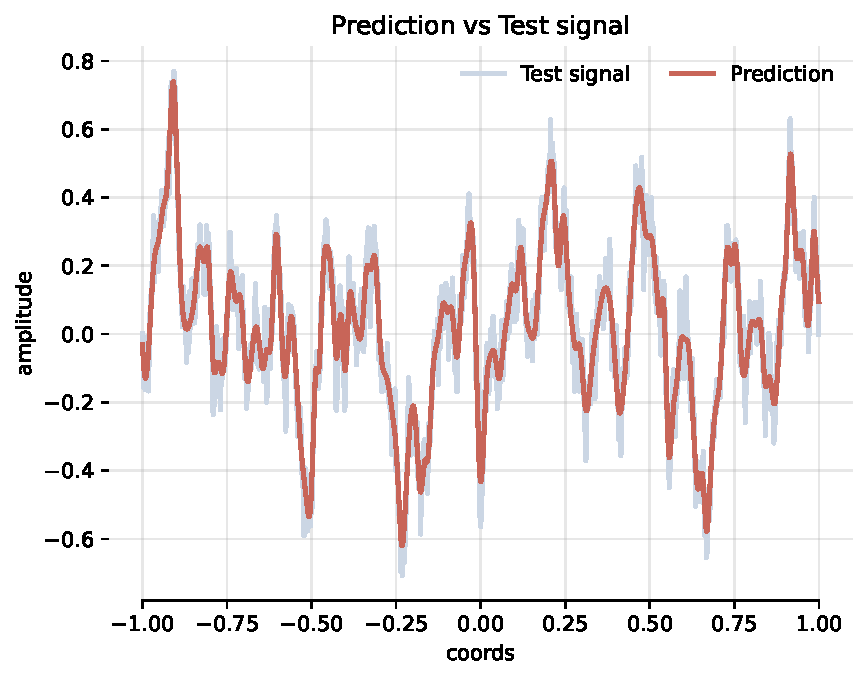
\includegraphics[width=\textwidth]{img/ch4/pred-noise-1hl-16hf-w8.pdf}
        \caption{16 neurons}
        \label{fig:pred-noise-1hl-16hf-w8}
    \end{subfigure}
    \begin{subfigure}[b]{0.32\textwidth}
        \centering
        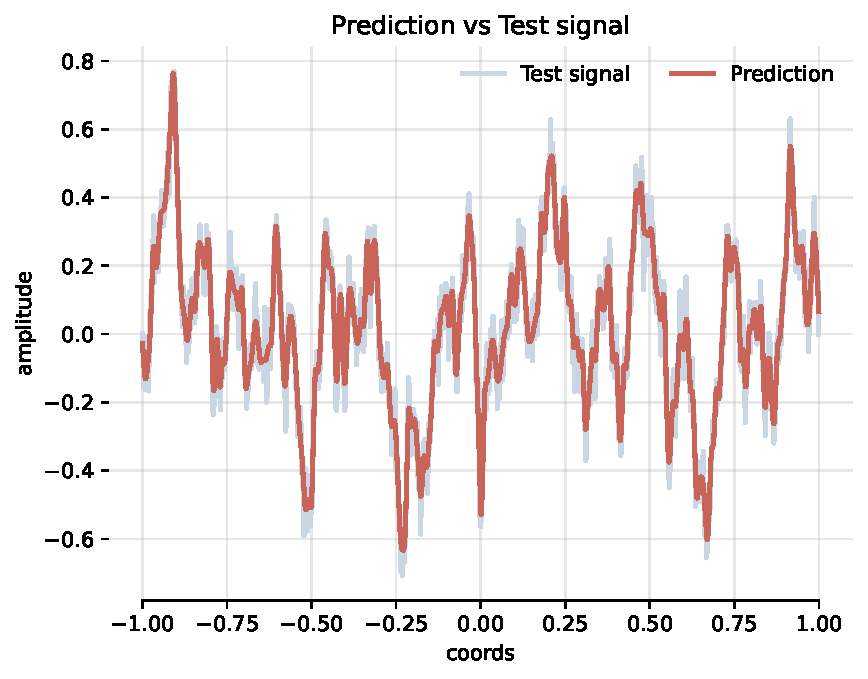
\includegraphics[width=\textwidth]{img/ch4/pred-noise-1hl-32hf-w8.pdf}
        \caption{32 neurons}
        \label{fig:comp-pred-noise-1hl-32hf-w8}
    \end{subfigure}
    \begin{subfigure}[b]{0.32\textwidth}
        \centering
        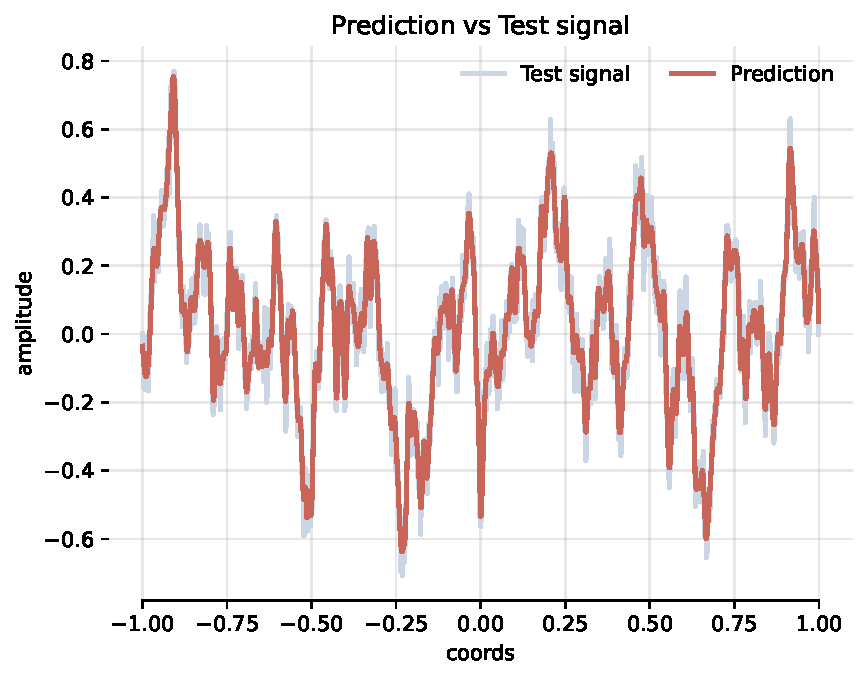
\includegraphics[width=\textwidth]{img/ch4/pred-noise-1hl-64hf-w8.pdf}
        \caption{64 neurons}
        \label{fig:pred-noise-1hl-64hf-w8}
    \end{subfigure}

    \begin{subfigure}[b]{0.32\textwidth}
        \centering
        \includegraphics[width=\textwidth]{img/ch4/4x-zoom-noise-1hl-16hf-w8.pdf}
        \caption{16 neurons}
        \label{fig:4x-zoom-noise-1hl-16hf-w8}
    \end{subfigure}
    \begin{subfigure}[b]{0.32\textwidth}
        \centering
        \includegraphics[width=\textwidth]{img/ch4/4x-zoom-noise-1hl-32hf-w8.pdf}
        \caption{32 neurons}
        \label{fig:comp-4x-zoom-noise-1hl-32hf-w8}
    \end{subfigure}
    \begin{subfigure}[b]{0.32\textwidth}
        \centering
        \includegraphics[width=\textwidth]{img/ch4/4x-zoom-noise-1hl-64hf-w8.pdf}
        \caption{64 neurons}
        \label{fig:4x-zoom-pred-noise-1hl-64hf-w8}
    \end{subfigure}

    \begin{subfigure}[b]{0.32\textwidth}
        \centering
        \includegraphics[width=\textwidth]{img/ch4/fft-noise-1hl-16hf-w8.pdf}
        \caption{16 neurons}
        \label{fig:fft-noise-1hl-16hf-w8}
    \end{subfigure}
    \begin{subfigure}[b]{0.32\textwidth}
        \centering
        \includegraphics[width=\textwidth]{img/ch4/fft-noise-1hl-32hf-w8.pdf}
        \caption{32 neurons}
        \label{fig:comp-fft-noise-1hl-32hf-w8}
    \end{subfigure}
    \begin{subfigure}[b]{0.32\textwidth}
        \centering
        \includegraphics[width=\textwidth]{img/ch4/fft-noise-1hl-64hf-w8.pdf}
        \caption{64 neurons}
        \label{fig:fft-noise-1hl-64hf-w8}
    \end{subfigure}
    \caption{Comparison between different network widths}
    \label{f:comparison-16-32-64-hf}
\end{figure}


If we keep the width of the network fixed and increase the range of frequencies used in the initialization, we can gradually capture higher frequencies. This happens until we reach the capacity of the network, when its performance starts to degenerate and the result becomes noise. Figure \ref{f:comparison-8-to-256-hz} illustrates this phenomenon with a network with 32 neurons per layer. Notice that from 8Hz to 64 Hz, the network gets better in capturing finer details of the signal. However, when $\omega_0=128$, the reconstruction presents peaks and valleys bigger than those present in the signal, a clear evidence of spurious frequencies. When $\omega_0=256$ the result totally degenerates into noise.

\begin{figure}[h]
    \centering
    \begin{subfigure}[b]{0.32\textwidth}
        \centering
        \includegraphics[width=\textwidth]{img/ch4/16x-zoom-1hl-32hf-8hz.pdf}
        \caption{$\omega_0=8$}
        \label{fig:16x-zoom-1hl-32hf-8hz}
    \end{subfigure}
    \begin{subfigure}[b]{0.32\textwidth}
        \centering
        \includegraphics[width=\textwidth]{img/ch4/16x-zoom-1hl-32hf-16hz.pdf}
        \caption{$\omega_0=16$}
        \label{fig:16x-zoom-1hl-32hf-16hz}
    \end{subfigure}
    \begin{subfigure}[b]{0.32\textwidth}
        \centering
        \includegraphics[width=\textwidth]{img/ch4/16x-zoom-1hl-32hf-32hz.pdf}
        \caption{$\omega_0=32$}
        \label{fig:16x-zoom-1hl-32hf-32hz}
    \end{subfigure}

    \begin{subfigure}[b]{0.32\textwidth}
        \centering
        \includegraphics[width=\textwidth]{img/ch4/16x-zoom-1hl-32hf-64hz.pdf}
        \caption{$\omega_0=64$}
        \label{fig:16x-zoom-1hl-32hf-64hz}
    \end{subfigure}
    \begin{subfigure}[b]{0.32\textwidth}
        \centering
        \includegraphics[width=\textwidth]{img/ch4/16x-zoom-1hl-32hf-128hz.pdf}
        \caption{$\omega_0=128$}
        \label{fig:16x-zoom-1hl-32hf-128hz}
    \end{subfigure}
    \begin{subfigure}[b]{0.32\textwidth}
        \centering
        \includegraphics[width=\textwidth]{img/ch4/16x-zoom-1hl-32hf-256hz.pdf}
        \caption{$\omega_0=256$}
        \label{fig:16x-zoom-1hl-32hf-256hz}
    \end{subfigure}
    \caption{Comparison between different ranges of frequencies in initialization}
    \label{f:comparison-8-to-256-hz}
\end{figure}

Repeating this experiment with more neurons per layer, we observe that we can use higher values of $\omega_0$ to correctly learn to represent the input signal (Figure \ref{f:comparison-64-to-256-hf}).


\begin{figure}[h]
    \centering
    \begin{subfigure}[b]{0.32\textwidth}
        \centering
        \includegraphics[width=\textwidth]{img/ch4/16x-zoom-1hl-64hf-128hz.pdf}
        \caption{64 neurons, $\omega_0=128$}
        \label{fig:16x-zoom-1hl-64hf-128hz}
    \end{subfigure}
    \begin{subfigure}[b]{0.32\textwidth}
        \centering
        \includegraphics[width=\textwidth]{img/ch4/16x-zoom-1hl-128hf-128hz.pdf}
        \caption{128 neurons, $\omega_0=128$}
        \label{fig:16x-zoom-1hl-128hf-128hz}
    \end{subfigure}
    \begin{subfigure}[b]{0.32\textwidth}
        \centering
        \includegraphics[width=\textwidth]{img/ch4/16x-zoom-1hl-256hf-128hz.pdf}
        \caption{256 neurons, $\omega_0=128$}
        \label{fig:16x-zoom-1hl-256hf-128hz}
    \end{subfigure}

    \begin{subfigure}[b]{0.32\textwidth}
        \centering
        \includegraphics[width=\textwidth]{img/ch4/16x-zoom-1hl-64hf-256hz.pdf}
        \caption{64 neurons, $\omega_0=256$}
        \label{fig:16x-zoom-1hl-64hf-256hz}
    \end{subfigure}
    \begin{subfigure}[b]{0.32\textwidth}
        \centering
        \includegraphics[width=\textwidth]{img/ch4/16x-zoom-1hl-128hf-256hz.pdf}
        \caption{128 neurons, $\omega_0=256$}
        \label{fig:16x-zoom-1hl-128hf-256hz}
    \end{subfigure}
    \begin{subfigure}[b]{0.32\textwidth}
        \centering
        \includegraphics[width=\textwidth]{img/ch4/16x-zoom-1hl-256hf-256hz.pdf}
        \caption{256 neurons, $\omega_0=256$}
        \label{fig:16x-zoom-1hl-256hf-256hz}
    \end{subfigure}
    \caption{Reconstruction of higher frequencies bigger capacity networks}
    \label{f:comparison-64-to-256-hf}
\end{figure}


By comparing the Fast Fourier Transform of the learned signal and the target signal, we conclude that the network learned the low frequencies of the signal up to an unknown value that increases or decreases with $\omega_0$.

\red{Investigate more the reconstruction quality in this case - maybe add some metrics?}

% as if we were reconstructing only its low frequencies. Again, when we plot the Fast Fourier Transform of both the original signal and its reconstruction, we verify that the low frequencies match indeed (Figure \ref{fig:fft-smooth-noise1}).} 






% \begin{figure}
%     \centering
%     \begin{subfigure}[b]{0.3\textwidth}
%         \centering
%         \includegraphics[width=\textwidth]{img/placeholder512.png}
%         \caption{$Ground truth$}
%         \label{fig:gt-noise1}
%     \end{subfigure}
%     \hfill
%     \begin{subfigure}[b]{0.3\textwidth}
%         \centering
%         \includegraphics[width=\textwidth]{img/placeholder512.png}
%         \caption{Reconstruction}
%         \label{fig:rec-smooth-noise1}
%     \end{subfigure}
%     \hfill
%     \caption{Reconstruction of a signal with high frequencies with a network inititialized with much lower frequencies}

%     \begin{subfigure}[b]{0.6\textwidth}
%         \centering
%         \includegraphics[width=\textwidth]{img/placeholder512.png}
%         \caption{Reconstruction in $[-1, 1]$}
%         \label{fig:fft-smooth-noise1}
%     \end{subfigure}

%     \label{f:noise-smoothed-reconstruction}
% \end{figure}

% We observe that as we increase the value of $\omega_0$, meaning the frequency interval used in initialization of the first layer of the sinusoidal network, it becomes better in fitting fine details of the signal. Figure \ref{f:zoomed-views-noise} shows some zoomed views of the reconstruction. The grid where the network has been evaluated \red{has been refined XX, XXX and XXXX times}. Note that the model is well behaved in the points that were not given as supervision (not part of the training data), that is, it correctly interpolates the signal.

% \begin{figure}
%     \centering
%     \begin{subfigure}[b]{0.3\textwidth}
%         \centering
%         \includegraphics[width=\textwidth]{img/placeholder512.png}
%         \caption{$Ground truth$}
%         % \label{fig:gt-noise1}
%     \end{subfigure}
%     \hfill
%     \begin{subfigure}[b]{0.3\textwidth}
%         \centering
%         \includegraphics[width=\textwidth]{img/placeholder512.png}
%         \caption{Reconstruction}
%         % \label{fig:rec-smooth-noise1}
%     \end{subfigure}
%     \hfill
%     \caption{Reconstruction of a signal with high frequencies with a network inititialized with much lower frequencies}
%     \begin{subfigure}[b]{0.3\textwidth}
%         \centering
%         \includegraphics[width=\textwidth]{img/placeholder512.png}
%         \caption{Reconstruction }
%         % \label{fig:fft-smooth-noise1}
%     \end{subfigure}
%     \label{f:zoomed-views-noise}
% \end{figure}


% On the other hand, if $\omega_0$ is too high it may cause the training to diverge. \red{In the Figure \ref{f:diverging-omega0}, we show the evolution of the training loss (Figure \ref{fig:diverging-loss}) and the result (Figure \ref{fig:diverging-reconstruction}) after 200 epochs when we initialized the SIREN with $\omega_0=600$. Note that after about 50 epochs, the loss starts to increase and our final result bears no resemblance to the original signal.}

% \begin{figure}
%     \centering
%     \begin{subfigure}[b]{0.3\textwidth}
%         \centering
%         \includegraphics[width=\textwidth]{img/placeholder512.png}
%         \caption{$Loss function$}
%         \label{fig:diverging-loss}
%     \end{subfigure}
%     \begin{subfigure}[b]{0.3\textwidth}
%         \centering
%         \includegraphics[width=\textwidth]{img/placeholder512.png}
%         \caption{Reconstruction}
%         \label{fig:diverging-reconstruction}
%     \end{subfigure}
%     \caption{Reconstruction of a signal with high frequencies with a network inititialized with much lower frequencies}
%     \label{f:diverging-omega0}
% \end{figure}

% \red{To achieve the result shown in the first figure, where the signal is perfectly fitted, we used $\omega_0 = 200$. We found that a value between $100$ and $200$ converges to a good approximation quickly (around 200 epochs). 

% \begin{figure}
%     \includegraphics[width=0.3\linewidth]{img/placeholder512.png}
%     \caption{Fitting of a regular signal using Siren initialization and their default suggested hyperparameters}
% \end{figure}


% We conclude that the frequency initialization of the first layer, which depends on $\omega_0$, is of central importance in the convergence of network training and multiresolution learning.
% Ideally we should initialize the network with frequencies that match the frequency content of the target signal. However, as we do not have access to this information in many applications, we must guess a value for $\omega_0$. Here, the Shannon-Nyquist therorem may help us bound the value of $\omega_0$. For example, considering a sampling rate of 512 Hz, we cannot represent frequencies higher than 256 (half the sampling rate), so it does not make sense to choose $\omega_0$ higher than this value. Also, since the composition of sines generates higher frequencies \cite{novello2022understanding}, it is reasonable to initialize the netowork with much lower frequencies than the Nyquist limit.


% Another point worth noticing is that if the initialization frequencies are too high, the hidden layers may generate even higher frequencies, and even a model with high capacity will introducing noise into the model's reconstruction. This noise is not evident at the training coodinates, as the model overfits this data well, but it can be observed in a more refined grid (Figure \ref{f:placeholder-ref}).

% \subsection{Capacity Filtering}

% So far, we have worked with a high capacity SIREN Network using 3 hidden layers with 256 units per layer. As we saw, this network can approximate our 1D signals perfectly and, in fact, we know it can approximate much more complex signals. For example, representations of neural implicit surfaces in three and higher dimensions.

% We decreased the number of layers and computational units to evaluate what happens when we try to approximate a signal using a SIREN model with lower capacity than it would be necessary. Experiments showed us that we can also reconstruct a filtered version of the target signal when using low capacity SIREN models initialized with small $\omega_0$.


% \section{The Multiresolution Module}

% Our goal is to design a module capable of approximating a signal with multiple frequency bands. When we introduce hidden layers, we know, from previous experiments, that the model capacity increases and we can’t control the exact content of frequencies the network learns. This way, we aimed for a module with a single hidden layer and used Perlin Noises with 4 local extrema (Figure 17) as a perceptual indicator of ”limited frequency band”.

% We did experiments with 1 and 2 hidden layers modules using 8, 16 or 32 computational units in each layer. After looking at the results, we chose a module with 1 hidden layer and 16 units in each layer as our MR-Module for most experiments.

% \begin{figure}
%     \centering
%     \begin{subfigure}[b]{0.3\textwidth}
%         \centering
%         \includegraphics[width=\textwidth]{img/placeholder512.png}
%         % \caption{$Loss function$}
%         % \label{fig:diverging-loss}
%     \end{subfigure}
%     \begin{subfigure}[b]{0.3\textwidth}
%         \centering
%         \includegraphics[width=\textwidth]{img/placeholder512.png}
%         % \caption{Reconstruction}
%         % \label{fig:diverging-reconstruction}
%     \end{subfigure}
%     \caption{Reconstruction of low frequency signals using a small size model}
%     \label{f:mr-module}
% \end{figure}

% We have not targeted the minimal module possible, as Figure XXX shows this module is able to approximate more complex signals up to a certain frequency. Having a small module with reasonable capacity gives us more flexibility in terms of level of detail strategy and helps to keep each stage of different MR-Net architectures uniformly as we will discuss on the next section. However, the breadth and depth of the MR-Module could be adapted to specific applications without compromising compatibility with the MR-Nets architectures.



% \section{Multiresolution Training}

% We have established that we can bound the frequencies learned by a sinusoidal neural network by adjusting the interval of frequencies sampled for initialization of its first layer, and also by adjusting the network capacity. That is, if the value of $\omega_0$ is too low, the network will learn the lower frequencies of the signal, fitting their intensities in the Fourier spectrum, but won't learn the higher frequencies, even if it has enough computational units to to do. On the other hand, if the capacity given by the computational units is too small, the result will also resemble a filtered version of the target signal.

% \subsection{Gaussian Pyramid Training}


% After exploring the impact of different values of initialization frequencies, we investigated if we could fit multiple scales of the same signal by building a Gaussian pyramid of it. We filtered the signal using a box filter of dimension 5, decimated it by a factor of 2 and used this subsampled version to train our network. Then, we used the trained network to predict the values over all originally sampled points, so we could verify its behaviour on unsupervised points. As we are filtering the higher frequencies of the signal, we expect to be able to represent it exactly by using fewer samples, acconding to the classical sampling theory.  
% We compared our result to a smoothed but not decimated version of the signal where we doubled the size of the filter as we walked to coarse scales. The panel of figures below shows the result of fitting a signal in 7 different scales, starting with \omega_0=256 and dividing it by 2 as we walk to coarse scales.
% We trained the network using less points at each scale.

% \begin{figure}[!htb]
% \minipage{0.49\textwidth}
% \includegraphics[width=\linewidth]{charts/Section-20-Panel-0-ulotlhctz}
% \caption{}
% \endminipage\hfill
% \minipage{0.49\textwidth}
% \includegraphics[width=\linewidth]{charts/Section-20-Panel-1-twwld6gku}
% \caption{}
% \endminipage
% \end{figure}

% For all the experiments until now, we used a SIREN with 3 hidden layers and 128 perceptrons in each layer, which seemed to be more than necessary to fit all signals we experimented. However, if we initialize the network with frequencies that are unsuitable for the signal, it will reflect on the quality of the regression. For instance, the figure below shows the difference between fitting a signal in the 6th scale using \omega_0=8 or \omega_0=16.

% \begin{figure}[!htb]
% \minipage{0.49\textwidth}
% \includegraphics[width=\linewidth]{charts/Section-22-Panel-0-ulotlhctz}
% \caption{}
% \endminipage\hfill
% \minipage{0.49\textwidth}
% \includegraphics[width=\linewidth]{charts/Section-22-Panel-1-twwld6gku}
% \caption{}
% \endminipage
% \end{figure}

% \section{Minimal Module}
% dsdsdsd

% \begin{figure}[!htb]
% \minipage{0.49\textwidth}
% \includegraphics[width=\linewidth]{charts/Section-26-Panel-0-rpuua88ix}
% \caption{}
% \endminipage\hfill
% \minipage{0.49\textwidth}
% \includegraphics[width=\linewidth]{charts/Section-26-Panel-1-z4g8njbpz}
% \caption{}
% \endminipage
% \end{figure}

% If we train for more epochs, it approximates better
% $\omega_0$ = 32
% 1 hidden layer; 16 hidden features
% Trained for 8 thousands epochs

% \begin{figure}[!htb]
% \minipage{0.49\textwidth}
% \includegraphics[width=\linewidth]{charts/Section-30-Panel-0-rpuua88ix}
% \caption{}
% \endminipage\hfill
% \minipage{0.49\textwidth}
% \includegraphics[width=\linewidth]{charts/Section-30-Panel-1-z4g8njbpz}
% \caption{}
% \endminipage
% \end{figure}

% \section{Visualizing the basis functions}
% dsdsdsdsdsdsdss
% \section{To be investigated}
% How should we connect the modules to train our network?


% \chapter{Multiresolution Sinusoidal Neural Networks}
% \label{ch:mrnet}

% In recent years, the computer science community has seen an explosion in research in neural networks, motivated mainly by advances in Deep Learning~\cite{lecun2015deep,goodfellow2016deep}.
% For visual computing, this was spurred by the creation of Convolutional Neural Networks~(CNNs)~\cite{cnn98}, which had a significant impact both for the research community and the society at large~\cite{li2021survey,shamsaldin2019study}.
% The effectiveness of CNNs comes from the translation invariant properties of the convolution operator, which makes it a proper architecture for the analysis of visual imagery.

% Deep neural networks such as CNNs, employ an array-based discrete representation of the underlying signal. In this case, the network input consists of a vector of pixel values (in RGB) representing the image \emph{directly} by data samples. We call this kind of network a \textit{data-based} network.


% Moreover, the revolution in the media industry caused by deep neural networks motivated the development of new image representations using neural networks. While the data-based network is appropriate for analysis tasks, relying on a discretization of the image, another kind of network called \textit{coordinate-based~network} is suitable for synthesis, and provides a continuous and compact representation. For its characteristics, there is a growing interest in using these networks in imaging applications~\cite{xie2022neural}.
% For instance, coordinate-based networks have been successfully applied in image compression~\cite{dupont2021coin} and super-resolution~\cite{czerkawski2021neural}.


% A coordinate-based network represents the image \emph{indirectly} using a fully connected \textit{multi-layer perceptron} (MLP) that takes as input a pixel coordinate and outputs a RGB color. These~networks provide a continuous implicit representation for images~\cite{chen2021learning}, and allow for various applications, from Neural Signed Distance Functions~(NeuralSDFs)~\cite{park2019deepsdf} to Neural Radiance Fields~(NeRFs)~\cite{mildenhall2021nerf}. Since the coordinates are continuous, images can be presented in arbitrary resolution.

% % Sinusoidal neural networks are particularly suited to model stationary or quasi-stationary signals due to the periodic nature of its activation function~\cite{chen2022}.

% Sinusoidal neural networks are examples of coordinate-based networks in which their activation function is the sine function. As such, they bridge the gap between the spatial and spectral domains, given the close relationship of the sine function with the Fourier~basis. However, these sinusoidal neural networks have been regarded as difficult to train~\cite{taming2017}. To overcome this problem, \citet{sitzmann2019siren} proposed a sinusoidal network for signal representation called SIREN. One of the key contributions of this work is the initialization scheme that guarantees stability and good convergence. Furthermore, it also allows modeling fine details in accordance with the signal’s frequency content.

% A \textit{multiplicative filter network} (MFN) is a sinusoidal network simpler than SIREN which is equivalent to a shallow sinusoidal network~\cite{fathony2020multiplicative}. \citet{bacon2021} presented \textit{band-limited coordinate network }(BACON), an MFN that produces intermediate outputs with an analytical spectral bandwidth (specified at initialization) and achieves multiresolution of the underlying signal. While its structure allows BACON to be expressed as a linear combinations of sines, avoiding the composition of sines present in sinusoidal MLPs, it creates multiresolution representations by truncating the frequency spectra of the signals. This approach produces ringing artifacts  in some levels of detail, and becomes evident when we look at the Fourier transform of the images.

% The control of frequency bands in the representation is closely related with the capability of adaptive reconstruction of the signal in multiple levels of detail.
% In that context, \citet{mueller2022instant} developed a multiresolution neural network architecture based on hash encoding. Also, \citet{martel2021acorn} designed an adaptive coordinate network for neural signals.

% In this context, we introduce \textit{multiresolution sinusoidal neural networks}~(MR-Net) based on classical signal multiresolution representations. 
% Our results, presented in Section~\ref{sub:spectra-eval}, indicate that using MR-Net produces better results compared to the previous state-of-the-art technique, BACON, while employing a smaller number of parameters.
% We describe three MR-Net subclasses: S-Net, L-Net and M-Net.
% Finally, we present applications on antialiasing and level-of-detail reconstruction.

% In summary, we make the following contributions:
% \begin{itemize}
%   \item We extend the sinusoidal neural networks and introduce a family of multiresolution coordinate-based networks, with unified architecture, that provides a continuous representation spatially and in scale. For this, we show how the initialization proposed for SIREN \cite{sitzmann2019siren} can be better explored to control the frequencies learned by the model, and how we can decompose a network in multiple stages, inspired by the multiresolution analysis.
%   \item We develop a framework for imaging applications based on this architecture, leveraging classical multiresolution concepts such as pyramids. Also, we show that this approach can more faithfully represent the frequency spectra of multiresolution signals, avoiding artifacts present in BACON \cite{bacon2021} representation.
%   \item We show that our architecture can represent images with good visual quality, being competitive with related methods in PSNR and number of parameters; we also demonstrate its use in applications of texture magnification and minification, and antialiasing. 
% \end{itemize}


% This paper is an extension of our previous work~\cite{paz2022}, where we introduced a class of neural networks called \textit{Multiresolution Neural Networks}~(MR-Net). In this work, we  present a complete description of this class of networks along with the motivations and a detailed mathematical model~(see Sec.~\ref{sec:mr_snn}). We added Section~\ref{sec:mrnet_detail}, which explains our framework in detail and should help the construction of an independent implementation. We expanded the comparisons to include an analysis of the frequency spectra of the representations provided by MR-Net and BACON (see Sec. \ref{sub:spectra-eval}). We also present a broader set of experiments (see Sec.~\ref{sub:kodak}), using the Kodak dataset~\cite{KodakDataset}, for comparison of the MR-Net with other network architectures. Finally, we added Section~\ref{sec:considerations}, which compares the different MR-Net subclasses~(S-Net, L-Net, and M-Net) in both qualitative and quantitative aspects.

% - Related Works: Mip-Nerf; Bacon; 

% \subsection{Signal Reconstruction from Multiresolution Representations }

% We leverage the knowledge from sinusoidal networks initialization and multiresolution theory to devise a multi-stage architecture for neural networks. 

% - Show how it is possible to reconstruct a signal from the Gaussian Pyramid using regular sampling.

% - \red{TODO: Show how it is possible to reconstruct a signal from the Laplacian Pyramid using regular sampling.}

% - Argument that we could build S-Net for completeness, which would be equivalent to a shallow sinusoidal network such as Bacon.

% - Show that multi-stages neural networks are equivalent to deep sinusoidal neural networks.


% \section{Multiresolution Sinusoidal Neural Networks}\label{sec:mr_snn}

% This section presents \emph{multiresolution sinusoidal neural networks} (MR-Net) to represent signals in multiple levels of detail using sinusoisal MLPs.


% \subsection{Overview of the MR-Net framework}

% Our proposal is a family of coordinate-based networks with an unified architecture, and a framework for training neural networks on multiscale signal representation. We derive three main subclasses of MR-Nets: \emph{S-Net}, \emph{L-Net}, and \emph{M-Net}. Each of them offers different trade-offs in terms of frequency control in the signal representation.

% The characteristics of the MR-Net framework are:

% \begin{itemize}

% \item Flexible training data -- the input signal can be given either by regular sampling, by multiresolution structure such as pyramids, or by stochastic / stratified sampling.

% \item 2 Types of Level of Detail -- when training with multiresolution data, the level of details are determined by spectral projections, whereas with a single-resolution input signal, the level of details are determined by the network capacity.

% \item Progressive Training -- the network is trained progressively, each stage at a time, using a variety of schedule regimes.

% \item Continuous Multiscale -- the representation is continuous both in space and scale. Therefore, it can reconstruct the signal at any desired resolution / level of detail.
% \end{itemize}


% The next sections present the motivations and concepts underlying our approach, as well as the MR-Net architecture.

% \subsection{Motivation}
% \label{s-motivation}
% Let $\gt{f}:\mathcal{D}\to \mathcal{C}$ be a \textit{signal}, the \textit{ground-truth}, where $\mathcal{D}$ and $\mathcal{C}$ are finite vector spaces representing the domain and codomain of~$\gt{f}$. For instance, to represent an image, we can choose $\mathcal{D}=\R^2$ to represent the image's support and $\mathcal{C}=\R^3$ to represent the RGB \textit{color space}.
% Throughout the text, the cursive letter will indicate the ground-truth while the standard letter indicates the corresponding neural network.


% We can decompose the signal into a sum $\gt{f}=\gt{g}_0+\dots+\gt{g}_{N-1}$ of $N$ stages, where $\gt{g}_0$ is its coarsest approximation and $\gt{g}_i$, for $i>0$, progressively introduce finer details. The \textit{level of detail}~$i$ is defined as 
% $\gt{f}_i\!=\!\gt{g}_0\!+\!\cdots\!+\!\gt{g}_{i}$, or as 
% $\gt{f}_i\!=\!\gt{f}\!-\left(\gt{g}_{i+1}\!+\!\cdots\!+\!\gt{g}_{N-1}\right)$. 
% Thus, the stages can be defined as
% $$\gt{g}_i=\gt{f}_{i+1}-K*\gt{f}_{i+1}, \text{ with } \gt{f}_{N-1}=\gt{f}.$$

% That is, each stage $\gt{g}_i$ is the difference between the level $i+1$ and its convolution with a low-pass filter $K$. For example, $K$ could be a \textit{Gaussian kernel} $G(x,t)=\frac{1}{2\pi t}\exp{(-\frac{\norm{x}^2}{2t})}$, where $t$ is the scale parameter. The sequences $\{\gt{f}_i\}$ and $\{\gt{g}_i\}$ resemble the \textit{Gaussian} and \textit{Laplacian pyramids}, which are widely used in the multiresolution analysis of digital images~\cite{rosenfeld2013multiresolution,lindeberg1994scale,velho2009image}.

% \pagebreak

% We address the problem of representing a signal $\gt{f}$ in multiresolution using sinusoidal neural networks.
% Motivated by the decomposition $\gt{f}=\gt{g}_0+\dots+\gt{g}_{N-1}$, we consider an aggregation of $N$ sinusoidal MLPs $g_i:\mathcal{D}\to \mathcal{C}$, which we call stages, to approximate $\gt{f}$. Therefore, we propose training each network stage $g_i$ by fitting it to the stages $\gt{g}_i$ of $\gt{f}$. This approach allows us to learn the frequency of $\gt{f}$ in a controlled manner, starting from lower details and gradually moving towards higher ones.
% % This is also inspired by the fact that MLPs tend to learn lower frequencies first, a phenomenon known as \emph{spectral bias}~\cite{Rahaman2018O}. 
% % We use a specific initialization of each network $g_i$ to control its capacity such that we can fit it to the stages $\gt{g}_i$ of $\gt{f}$.

% % and as the training advances we add the the stages advances we consider 

% % use the  that increasing the network depth (for fixed width) improves the network’s ability to fit higher frequencies, while increasing the width (for fixed depth) also helps, but the effect is considerably weaker.



% \subsection{MR-Net Architecture}

% We define the MR-Net as a function $f:\mathcal{D}\times [0,N]\to \mathcal{C}$, expressed as follows:
% \begin{align}\label{e-mrnet}
% f(x,t) = c_0(t)g_0(x) + \cdots + c_{N-1}(t)g_{N-1}(x),
% \end{align}
% Each function $g_i:\mathcal{D}\to\mathcal{C}$ is a sinusoidal MLP (see Sec~\ref{s-mr-module} for its precise definition) and represents the $i$th \textit{stage} of $f$, whose contribution is controlled by the function 
% \begin{align}\label{e-control}
% c_i(t)=\max\Big\{0, \min\big\{1, t-i\big\}\Big\}.
% \end{align}
% Note that when $t<i$, $c_i(t)=0$; when $i\leq t\leq i+1$, $c_i(t)=t-i$; and when $t>i+1$, $c_i(t)=1$.
% Therefore, if $t=k+\delta$ with $k\in\mathbb{N}$ and $0\leq\delta\leq 1$, we obtain $$f(x,t)=g_0(x)+\dots + g_k(x)+\delta g_{k+1}(x).$$ 
% $f_t:=f(\cdot, t):\mathcal{D}\to \mathcal{C}$ is the \textit{level of detail} $t$ of the MR-Net~$f$.
% These levels evolve continuously, allowing us to encode a continuous multiresolution of $f$ at full resolution $f_N\!=\!g_0+\cdots + g_{N-1}$.
% For this, we propose fitting $f$ to the multiresolution given by the ground-truth signal $\gt{f}=\gt{g}_0+\dots+\gt{g}_{N-1}$.
% We initialize the parameters of each stage $g_i$ with sufficient capacity to fit the stage $\gt{g}_i$ (see Sec~\ref{s-frequency-control}), then train each $g_i$ to approximate $\gt{g}_i$.

% The resulting MR-Net $f$ learns the decomposition of the ground-truth signal $\gt{f}$ as a projection into the coarse scale space and a sequence of finer detail spaces. For instance,
% the initial stage $f_1=g_0$ provides the least detailed approximation~of~$f_N$. The subsequent stages, represented by $g_i$ with $i<0$, progressively introduce finer details and are regulated by the scale parameter $t$. 
% Essentially, the multiresolution can be navigated using the scale parameter $t$ within the interval $[0,N]$, which makes this architecture closely aligned with the Multiresolution Analysis~\cite{mallat-mr89}.
% Fig~\ref{f:mrnet-arch} shows the structure of a MR-Net having $N$ stages. 
% \begin{figure}[!h]
% \centering
% \includegraphics[width=0.96\linewidth]{MRNet-CAG/new-figs/mr-net-stages-v2.png}
% \caption{Anatomy of the MR-Net Family.}
% \label{f:mrnet-arch}
% \end{figure}



% % The stages of the network are trained based on a predefined schedule (see Section~\ref{s:training}).
% % During training, the control layer is the identity function, i.e. $\alpha = 1$.  


% % The contributions of these $N$ stages are added together forming the network output.
% % Assuming that the MR-Net is learning a function $f(x)$ that fits the input signal, then
% % \begin{equation}
% %     f(x) = g_0(x) + \cdots + g_{N-1}(x)
% % \end{equation}
% % where $g_i(x)$ is the detail function representing the stage $i$.
% % The first stage $g_0$ gives the coarsest approximation of the signal and the other subsequent stages add increasingly finer details to it.





% % Note that this architecture is very much in the spirit of the Multiresolution Analysis~\cite{mallat-mr89}. Indeed, consider the base case with $f = g_0 + g_1$, then $g_1 = f - g_0$, i.e. $g_1$ are the details that need to be added to $g_0$ to increase the level of detail.

% % \hl{MR-Net learns the decomposition of the signal as a projection into the coarse scale space and a sequence of finer detail spaces.}
% %

% \subsection{MR Module}
% \label{s-mr-module}
% Each stage $g_i$ of the MR-Net $f$ is a sinusoidal MLP, called \textit{MR-Module}, that learns a signal representation as a combination of sinusoidal functions with induced frequency band.

% We write each stage as $g_i=L_i\circ H_i\circ S_i$. The first layer projects the input $x$ into a list of sines $S_i(x)$, which is the input of the composition $H_i$ of the MLP hidden layers. The output $H_i\circ S_i(x)$ is a dictionary of sine combinations that are passed to the linear layer $L_i$. Finally, the control layer $c_i(t)$, with $t\in[i,i+1]$, blends the stage $g_i$ with the level of detail $f(x,i-1)$. 

% There are two kinds of MR-Modules: \emph{Pure sine} MR-Module ($H_i=\emptyset$) and \emph{modulated sine} MR-Module ($H_i\neq\emptyset$). In the first case the network has only the first layer and the linear layer, and in the second case the network has the three blocks, including the hidden layers (see Fig~\ref{f:mr-module}).
% \begin{figure}[!h]
% \centering
% % \includesvg[width=\linewidth]{svg_figs/diagram_mrnet.svg}
% \includegraphics[width=\linewidth]{figs/diagram_mr_module.pdf}
% \caption{General Anatomy of a MR-Module.}
% \label{f:mr-module}
% \end{figure}

% Without loss of generality, let us assume that the ground-truth signal is a grayscale image unless stated to the contrary. In this case, the stages of the MR-Net will have $\R^2$ and $\R$ as domain and codomain respectively. 
% Consequently, a MR-Net with $N$ stages $g_i:\R^2\to \R$ has the form $f:\R^2\times [0,N]\to \R$.
% Under this assumption, we present the building blocks of the MR-Net with details. 


% \subsubsection{Pure Sine MR-Module}

% The pure sine MR-Module is a shallow sinusoidal MLP defined as the composition $L\circ S$ of a sinusoidal layer $S$ with a linear layer $L$.
% The layer $S\!:\!\R^2\!\to\! \R^m$ projects the input $x$ into a dictionary of $m$ sines of the form $S(x)=\sin\left(W_s x+ b_s\right)$, where $W_s\in \R^{m\times 2}$ and $b_s\in \R^{m}$ are the \textit{weight matrix} and \textit{bias}. The integer $m$ is the \textit{width} of the MR-Module.
% The layer $L\!:\!\R^m\!\to\! \R$ is an affine map $L(x)=W_lx+b_l$, where $W_l\in \R^{1\times m} $ and $b_l\in \R$  are the final weight matrix and bias.
% Hence, $L\circ S$ acts as a spectral filter controlled by the initialization of $W_s$.


% Since the risk landscape for the network loss has many local minima, it is expected that the weights $W_s$ can’t move much further than their initialization. Therefore, $W_s$ determine the range of frequencies one can filter from the input signal. Fig~\ref{f:pure-sine} shows the structure of the $L\circ S$ and an example of a signal consisting of a linear combination of two frequencies. In this example, we have the layers $S\!:\!\R\!\to\! \R^2, S(x) = (sin(x), sin(5x))$ and $L\!:\!\R^2\!\to\! \R, L(x_1, x_2) = x_1 + x_2$.
% \begin{figure}[!h]
% \centering
% \includegraphics[width=0.8\linewidth]{figs/pure-sine.png}
% \caption{Pure sine MR-Module.}
% \label{f:pure-sine}
% \end{figure}


% \subsubsection{Modulated sine MR-Module}

% The Modulated MR-Module is a deep sinusoidal MLP $L\circ H\circ S$ that considers a hidden sinusoidal layer block $H:\R^m\to~\R^m$. 
% This map is the composition of $k$ layers $H=H_k\circ \dots \circ H_1$ with $H_i(x_i)\!=\!\sin\left(W_i x_i \!+\! b_i\right)\!=\!x_{i+1}$ where $x_0\!\in\!\R^m$ is the input.
% The integers $m$ and $k+1$ are the \textit{width} and \textit{depth} of the MR-Module.  

% The MR-Module $L\circ H\circ S$ is a linear combination of a dictionary of (spectral) atoms $H\circ S$ containing composition of sines. This fact has two consequences. First, the capacity of $L\circ H\circ S$ is greater than the capacity of $L\circ S$ with the same number of neurons~\cite{novello2022understanding}. Second, the initialization of $L\circ H\circ S$ does not directly control its frequency band as in the case of $L\circ S$.

% In terms of localization properties in space and frequency, we can say the spectral atoms of the Modulated MR-Module are semi-local in the sense that these functions are adapted by the learning process to fit local variations of the signal (i.e., frequencies) across its (spatial) domain. This characteristic is evident in Fig~\ref{f:modulated} that shows a network structure and the graph of $\sin\Big(3\sin\big(5\sin(1.9x)\big)\Big)$.
% In this example, the first layer is represented by $S(x)=\sin(1.9 x)$, the hidden block is the composition of two sine layers $H(x)=\sin\big(3\sin(5x)\big)$, and the linear layer is the identity function $L(x)=x$.

% \begin{figure}[!h]
% \centering
% \includegraphics[width=0.9\linewidth]{figs/modulated-sine.png}
% \caption{Modulated sine MR-Module.}
% \label{f:modulated}
% \end{figure}



% \subsection{MR-Net Subclasses}

% Here, we describe three subclasses of the MR-Net: \emph{S-Net}, \emph{L-Net}, and \emph{M-Net}.
% The characteristics of their level of details depend on the configuration of their stages. %, as will be presented next.
% Recall, from Eq~\ref{e-mrnet}, that a MR-Net is a function $f:\R^2\times [0,N]\to \R$, expressed as:
% \begin{align*}
% f(x,t) = c_0(t)g_0(x) + \cdots + c_{N-1}(t)g_{N-1}(x).
% \end{align*}
% Therefore, to define the subclasses S-Net, L-Net, and M-Net, we only need to define the stages $g_i$.


% \subsubsection{S-Net}

% A S-Net is a MR-Net in which each stage $g_i$ is a pure sine MR-Module, i.e. $g_i=L_i\circ S_i$ where $S_i$ and $L_i$ are the first and the linear layers (see Fig~\ref{f:s-net}).
% %
% For this reason, each stage $g_i$ can be  
% % consists of a learned ``sine transform'', with its layers corresponding, respectively, to the direct and inverse sine transform. Specifically, 
% expressed as a sum of sine functions
% $$g_i(x)=a_0+\sum_{j=1}^m a_j \sin\left(\omega_j x+\varphi_j\right),$$ where the \textit{frequencies} $\omega_j$ and \textit{phase-shifts} $\varphi_j$ are given by the weights and bias of the first layer $S_i$. The \textit{amplitudes} $a_j$ are given by the linear layer $L_i$.
% %
% As a consequence, the resulting S-Net $f$ can provide level of detail based on the controlled initialization of frequency band of each stage $g_i$ (see Sec~\ref{s-frequency-control}).
% \begin{figure}[!h]
% \centering
% \includegraphics[width=0.58\linewidth]{MRNet-CAG/pdf_figs/snet.pdf}
% \caption{S-Net architecture.}
% \label{f:s-net}
% \end{figure}

% \subsubsection{L-Net}
% \label{s-lnet}
% A L-Net is a MR-Net $f$ in which each stage $g_i=L_i\circ H_i\circ S_i$ is an independent modulated sine MR-Module: $S_i$, $H_i$, $L_i$ are the first, hidden, and linear blocks (see Fig~\ref{f:l-net}).
% %
% For this reason, the level of detail capacity of $f$ is determined by the width and depth of each stage $g_i$.
% % The first stage $g_0$ is the coarsest approximation of the underlying function.
% \begin{figure}[!h]
% \centering
% \includegraphics[width=0.7\linewidth]{MRNet-CAG/pdf_figs/lnet.pdf}
% % \vspace{-0.4cm}
% \caption{L-Net architecture. Note that the stages are independent of each other.}
% \label{f:l-net}
% \end{figure}


% The $N$th level $f(\cdot, N)$ of a L-Net is an example of a sinusoidal MLP.
% Without loss of generality, let $f(\cdot, t)=~c_0(t)g_0+c_1(t)g_1$ be a L-Net with two stages having the same architecture with a single hidden layer. We show that $f(\cdot, 2)\!=\!L\!\circ\! H\!\circ\! S$.
% For this, define the matrices of $S$, $H$, and $L$, respectively, using $W_s\!=\!\begin{psmallmatrix}W_s^0\\W_s^1\end{psmallmatrix}$, 
% $W_h\!=\!\begin{psmallmatrix}W_h^0& 0\\0&W_h^1\end{psmallmatrix}$, 
% $W_l\!=\!\begin{psmallmatrix}W_l^0 & W_l^1\end{psmallmatrix}$, where $W_s^j$, $W_h^j$, $W_l^j$ are the matrices of the stages~$g_j$. The biases are defined in a similar way. Such procedure can be extended to a sum of $N$ stages in a analogous way.
% Thus, the L-Net gives us a controllable way of increasing the \textit{width} of a sinuoisal MLP during training.


% \subsubsection{M-Net}
% \label{s-mnet}
% While the stages of S-Nets and L-Nets are independent, with M-Net we propose a way to reuse information learned at previous stages.
% A M-Net is a MR-Net where each stage $g_i$ is a modulated MR-Module linked to its subsequent stage $g_{i+1}$.
% That~is, $H_i\circ  S_i$ is composed both with the linear layer $L_i$, producing the stage $g_i\! =\! L_i\!\circ\! H_i\!\circ\!  S_i$, and the hidden block $H_{i+1}$ resulting in $g_{i+1}\! =\! L_{i+1}\!\circ H_{i+1}\!\circ\left(S_{i+1}, H_i\circ  S_i\right)$ (Fig~\ref{f:m-net}).
% This way, the hidden block has the form $H_{i+1}\!:\!\R^{2m}\!\to\! \R^m$; $m$ is the number of neurons.
% \begin{figure}[!h]
% \centering
% \includegraphics[width=0.75\linewidth]{MRNet-CAG/pdf_figs/mnet.pdf}
% % \vspace{-0.4cm}
% \caption{M-Net architecture. Notice how the hidden-layers blocks of adjacent MR-Modules are connected.}
% \label{f:m-net}
% \end{figure}

% The hidden block of a stage of the M-Net is composed~with~a sequence of hidden blocks coming from previous stages.~That~is, the M-Net contains a deep MLP $L_{N-1} \circ \overline{H_{N-1}} \circ \cdots \circ \overline{H_1}\circ H_0 \circ S_0$ with $N$ hidden blocks; $\overline{H_i}$ is the part of $H_i$ connecting to the stage $g_{i+1}$.
% Thus, the M-Net also allows us to increase the \textit{depth} of a sinusoidal MLP during training implying that the capacity of each stage increases with its depth in the hierarchy.
% This feature makes the M-Net a suitable and compact architecture for  multiresolution training, as discussed in Sec~\ref{sec:considerations}, and we will utilize this subclass in the applications of Sec~\ref{s:img}.


% \subsection{Frequency Control}
% \label{s-frequency-control}

% Let $\gt{f}=\gt{g}_0+\cdots+\gt{g}_{N-1}$ be the ground-truth signal in multiresolution, and $f:\R^2\times [0,N]\to \R$ be a MR-Net with $N$ stages. To train each stage $g_i$, we propose to initiate its parameters based on the frequency content of $\gt{g}_i$.
% There are two ways to control the frequency band of $g_i$. First, we can initialize the weight matrix of the first layer of $g_i$. Second, we can vary its width and depth. Moreover, these mechanisms can be combined.


% \subsubsection{Frequency Initialization}
% \label{s-frequency-initialization}


% Training sinusoidal MLPs can be challenging  as periodic activation functions may lead to instability in deep architectures~\cite{taming2017}. \citet{sitzmann2019siren} propose an initialization scheme that guarantee stability during training. 
% They initialize the weights $W=\omega \, \tilde{W}$ of the MLP first layer $ \sin\left(Wx + b\right)$ such that $\tilde{W}$ is uniformly sampled in $[-1,1]$ and the number $\omega$ controls the range of frequencies. That is, the layer projects the input $x$ in a list of sines with frequencies in $[-\omega, \omega]$. 
% They empirically choose $\omega=30$ in their experiments. For the hidden layers, they choose the weights distributed uniformly in $\left(-\sqrt{6/m}, \sqrt{6/m}\right)$, where $m$ is the width of the layer. See \cite{sitzmann2019siren} for the details.

% Regarding the initialization of the MR-Net $f$, let $g_i=L_i\circ H_i\circ S_i$ be its $i$th stage, where $S_i$, $H_i$, and $L_i$ are its first, hidden, and linear blocks.
% Observe that each coordinate of the sinusoidal layer $S_i(x)=\sin\left(W_{s_i} x+b_{s_i}\right)$ has the form $\sin(\omega_1 x_1 +\omega_2 x_2 + \varphi)$, where the \textit{frequencies} $\omega_1$ and $\omega_2$ form a line of the matrix $W_{s_i}$, $x=(x_1,x_2)$ is the input, and the \textit{phase-shift} $ \varphi$ is a coordinate of the bias $b_{s_i}$. We follow the above initialization approach to initialize $g_{i}$. However, instead of using $\omega=30$ we consider it to be a \textit{bandlimit frequency} on the ground-truth stage $\gt{g}_i$.

% % The initialization of the elements of the matrix $W_{s_i}$ in the sinusoidal layer $S_i(x)=\sin\left(W_{s_i} x+b_{s_i}\right)$ is of central importance in the training convergence of $f$.

% Ideally, the initialization of frequencies in $g_i$ should match the frequency content of the ground-truth signal at the stage $\gt{g}_i$. 
% However, as we usually don’t have access to this information, we opt to use an upper bound. 
% Specifically, we assume that $\gt{g}_i$ has no frequency higher than a \textit{bandlimit} $B_i$. The Nyquist–Shannon sampling theorem says that we can reconstruct $\gt{g}_i$ from a sample $\{\gt{g}_i(x_{kl})\}$, where the regular grid $x_{kl}$ has points spaced with size $\frac{1}{r_i}<\frac{1}{2B_i}$. The number $r_i$ is the \textit{sample rate}. Fig~\ref{f:niquist} illustrates such requirement using the frequency rate notation.  
% % Assuming that the signal has been properly sampled, the ``Nyquist limit'' gives the maximum frequency contained in the signal, which is $\frac{1}{2} f_s$, where $f_s$ is the sampling rate (see Fig~\ref{f:niquist}).
% \begin{figure}[!h]
% \centering
% \includegraphics[width=0.7\linewidth]{figs/niquist.png}
% \vspace{-0.3cm}
% \caption{Nyquist Limit.}
% \label{f:niquist}
% \end{figure}


% Therefore, to fit the stage $g_i$ to the sample $\{\gt{g}_i(x_{kl})\}$, we opt to initialize $g_i$ such that it can represent frequencies up to $\omega_i:=\frac{r_i}{2}$.
% For this, we initialize the lines of the first matrix $W_{s_i}$ of $g_i$ uniformly in the set $\Omega_i=\left[-\omega_i, \omega_i\right]^2$.
% Thus, the sinusoidal layer $S_i$ may contain frequencies already initialized at previous stages because $\{\gt{g}_i\}$ is a Laplacian pyramid of $\gt{f}$, thus, $\Omega_0\subset \cdots \subset \Omega_{N-1}$. The weights of the hidden block $H_i$ are initialized following the same scheme in \cite{sitzmann2019siren}.

% % \vspace{0.2cm}
% % {\color{red}
% % In practice, we assume that the data is given as a regular sample (digital image) of size $2^{k}\times 2^k$
% % of the ground-truth signal~$\gt{f}$.
% % We abuse the notation by denoting this digital image by~$\gt{f}$.
% % To train the MR-Net stages~$\{g_i\}$, we use the (discrete) \textit{Gaussian} and \textit{Laplacian} pyramids of $\gt{f}$, both with $N<k$ levels.
% % Precisely, the Gaussian pyramid $\{\gt{f}_i\}$ is defined recursively by convolving the \textit{level of detail} $\gt{f}_i$ with a Gaussian kernel $K$ and downsampling the result by a factor 2:
% % \begin{align*}
% %     \gt{f}_i(k,l)&=\left(K*\gt{f}_{i+1}\right)(2k,2l)\,\, \text{with} \,\, k,l\in \left\{1,\ldots, 2^{k-N+1+i}\right\},\\
% %     \gt{f}_{N-1}&=\gt{f}.
% % \end{align*}
% % $\gt{f}_i(k,l)$ denotes the digital image $\gt{f}_i$ evaluated at the pixel $(k,l)$.
% % Similarly, the Laplacian pyramid $\{\gt{g}_i\}$ is defined using
% % \begin{align*}
% %     \gt{g}_i(k,l)&=\left(\gt{f}_{i}-K*\gt{f}_{i}\right)(2k,2l)\,\, \text{with} \,\, k,l\in \left\{1,\ldots, 2^{k-N+1+i}\right\}\\ \gt{g}_0(k,l)&=\left(K*\gt{f}_{1}\right)(2k,2l).
% % \end{align*}
% % Since $2^{k-N+1+i}$ is the height and width of $\gt{g}_i$, it cannot contain frequencies higher than $\omega_i=2^{k-N+i}$. 
% % Thus we propose to initialize the frequencies of the $N$ stages $\{g_i\}$ of the MR-Net $f$ following a dyadic sequence of frequency bands 
% % \begin{align}
% % \omega_{N-1}, \omega_{N-2}, \ldots, \omega_{0}.
% % \end{align}
% % Which is equivalent to $\omega_{N-1}, \frac{\omega_{N-1}}{2}, \ldots, \frac{\omega_{N-1}}{2^{N-1}}$ with $\omega_{N-1}= 2^{k-1}$.
% % These are the bandlimits used to define the sets $\Omega_i=\left[-\omega_i, \omega_i\right]^2$ to initialize the frequencies of the first layer of each stage $g_i$.
% % (see Fig~\ref{f:freq-bands}).

% % \begin{figure}[!h]
% % \centering
% % \includegraphics[width=0.98\linewidth]{figs/freq-bands.png}
% % \caption{Frequency Bands}
% % \label{f:freq-bands}
% % \end{figure}

% % }

% % Finally, the training of each stage $g_i$ is done by minimizing the following loss functional
% % \begin{align}
% %     \mathscr{L}(\theta_i)=\sum_{k=1}^{2\omega_i}\sum_{l=1}^{2\omega_i}\Big(\gt{g}_i(k ,l)-g_i(k,l)\Big)^2
% % \end{align}

% \subsubsection{MR-Module Capacity}
% \label{sec-module-capacity}

% The capacity of each MR-Net stage $g_i=L_i\circ H_i\circ S_i$ is controlled by its width $m$ and depth $k+1$.
% The width $m$ determines that an input $x$ will be transformed into a list of $m$ sines $S_i(x)=\sin\left(W_{s_i}x+b_{s_i}\right)$,
% where $W_{s_i}$ has rows sampled at the set $\Omega_i$ defined in Section~\ref{s-frequency-initialization}. By increasing $m$, the dictionary of input frequencies is augmented. The hidden block $H_i$ consisting of $k$ sinusoidal layers, further enhances this list of frequencies.

% Regarding the training of the MR-Net stage $g_i$, we recall that it is a MLP. \citet{Rahaman2018O} shows that during training a MLP learns lower frequencies first, a phenomenon known as \emph{spectral bias}. They also show that increasing the network depth (for fixed width) improves the network’s ability to fit higher frequencies, while increasing the width (for fixed depth) also helps, but the effect is considerably weaker. 


% To mitigate the effects of the spectral bias, we employ the above frequency initialization approach to the stage $g_i$. This ensures that the training of $g_i$ begins with frequencies that are \textit{close} to those present in the corresponding ground-truth data $\gt{g}_i$.
% % See Fig~\ref{f:capacity}.
% % \begin{figure}[!h]
% % \centering
% % \includegraphics[width=0.97\linewidth]{figs/width.png}\\
% % \includegraphics[width=0.97\linewidth]{figs/depth.png}
% % \vspace{-0.2cm}
% % \caption{Capacity Hyperparameters (from~\cite{Rahaman2018O})}
% % \label{f:capacity}
% % \end{figure}

% Furthermore, the MR-Net architecture enables us to gradually increase its width and depth by adding stages (see Secs~\ref{s-lnet} and \ref{s-mnet}), providing us with a controlled way of increasing network capacity while allocating ground-truth frequencies across stages in a controllable manner.
% For example, a L-Net can be viewed as a specific MLP where adding a new stage increases its width. As a result, L-Net allows us to divide a given MLP into stages. On the other hand, M-Net has a more sophisticated structure, as adding a stage results in a network that is wider and deeper.


% \section{MR-Net in Detail}
% \label{sec:mrnet_detail}

% This section presents the MR-Net framework in detail by conceptually dividing it in four main components: \emph{MR-Structure}, \emph{MR-Stages}, \emph{MR-Training}, and \emph{MR-Inference} (see Fig~\ref{f:components}). 

% % Although coordinate-based networks could be applied to represent signals in other dimensions, as demonstrated by SIREN \cite{sitzmann2019siren} and BACON \cite{bacon2021}, we are going to focus on images, that is signals XXXXX, the applications described in section XXXXX. For 1D applications, please refer to XXXXX.

% \begin{figure}[!h]
% \centering
% \includegraphics[width=0.99\linewidth]{figs/mr-net-components.png}
% \vspace{-0.3cm}
% \caption{MR-Net framework Components.}
% \label{f:components}
% \end{figure}

% Let $\gt{f}:\mathcal{D}\to \mathcal{C}$ be the ground-truth signal (\textit{input data}), and $f\!:\!\mathcal{D}\!\times\! [0,N]\!\to\! \mathcal{C}$ be a MR-Net with $N$ stages $\{g_i\}$ to fit $\gt{f}$~in multiresolution.
% We use this setting to present the framework.

% \subsection{MR-Structure}\label{sec:mr_struct}

% The MR-Structure is a data structure that encapsulates the input data $\gt{f}$. It includes $\gt{f}$ and metadata about its \textit{sampling mode}, \textit{filtering type}, and the \textit{multi-stage stack} (see Fig~\ref{f:structure}).
% \begin{figure}[!h]
% \centering
% \includegraphics[width=0.89\linewidth]{figs/mr-structure.png}
% \vspace{-0.4cm}
% \caption{MR-Structure.}
% \label{f:structure}
% \end{figure}

% % \subsubsection{Input Data}

% The training of MR-Net stage $g_i$ receives pairs $\{x_j, y_j\}$ as input, with points $x_j$ sampled in the domain $\mathcal{D}$ of $\gt{f}$ and $y_j=\gt{f}(x_j)\in~\mathcal{C}$. For a squared image, we could have $\mathcal{D}=[-1, 1]^2 \subset \R^{2}$. During training, we consider the signal $\gt{f}$ to have codomain in monochromatic ($\mathcal{C}=\R$) or RGB color ($\mathcal{C}=\R^3$) (see Fig~\ref{f:values}). 
% Depending on the application, other color spaces or additional attributes, such as masks and features, could be used (see Fig~\ref{f:attributes}). 
% \begin{figure}[!h]
% \centering
% \includegraphics[width=0.8\linewidth]{figs/attrib-d0-d1.png}
% \vspace{-0.2cm}
% \caption{Image values (RGB and monochromatic).}
% \label{f:values}
% \end{figure}

% \begin{figure}[!h]
% \centering
% \includegraphics[width=0.8\linewidth]{figs/attrib-mask.png}
% \vspace{-0.2cm}
% \caption{Examples of image attributes (mask and edges).}
% \label{f:attributes}
% \end{figure}


% The data input for the training of each of the $N$ stages $g_i$ is organized in a \textit{multi-stage stack} $\{x_j, y_j\}_i$.
% % consisting of a hierarchy of sampling grids. 
% Specifically, for each $i$, the set of pairs $\{x_j, y_j\}_i$ is a sample of the $i$th level of detail $\gt{f}_i$ of the signal $\gt{f}$ or a sample of the original signal $\gt{f}$, with $\{x_j\}_i\subset \mathcal{D}$ and $\{y_j\}_i=\{\gt{f}_i(x_j)\}$. 
% From the point of view of \textit{representation theory}, we can interpret this as a projection of the function $\gt{f}_i$ onto the primal \textit{Shannon basis} (i.e., Dirac delta distribution). In the context of signal processing, this basis is a sampling grid of impulses and the representation consists of the sequence $\{y_j\}_i$ at the grid locations $\{x_j\}_i$.

% \pagebreak

% The type of sampling used to extract the multi-stage stack $\{x_j, y_j\}_i$ from the signal $\gt{f}$ is an important aspect in the MR-Net training. In that respect, it is instrumental to consider two types of samplings: \textit{regular} and \textit{irregular} (Fig~\ref{f:sampling}). 
% %
% In the regular case, the sampled points are organized in a regular grid discretization $\{x_{k,l}\}$ of the domain $\mathcal{D}$. \comment{The irregular sampling consider the points $\{x_i\}$ to be uniformly sampled from $\mathcal{D}$.}
% % , i.e. for each pair $k,l$ we have $\norm{x_{k,l}-x_{k+1,l}}=\norm{x_{k,l}-x_{k,l+1}}=\Delta$ with $\Delta$ being a constant. 
% %
% For flexibility, we implement a sampler module that take regular samples or stochastic samples using the Poisson disk sampling~\cite{stochastic_cook, poisson_bridson}. 
% % The sampler could be extended to work with different sampling patterns. 
% % The sampling mode is stored in the MR-Structure, so it can be taken into account when doing operations that modify the sampling grid.

% \begin{figure}[!h]
% \centering
% \includegraphics[width=0.45\linewidth]{figs/regular.png}
% \hfil
% \includegraphics[width=0.45\linewidth]{figs/poisson.png}
% \\
% {\small\hfil (regular grid) \hfil\hfil\hfil (irregular grid) \hfil}
% \vspace{-0.2cm}
% \caption{Sampling modes.}
% \label{f:sampling}
% \end{figure}


% The multi-stage stack of the input signal $\gt{f}$ could have different resolutions.
% For the regular case where the sampled points are organized in a regular grid $\{x_{k,l}\}$ (the highest resolution), we can structure the multi-stages in dyadic lattice following the $2^i$ rule: 
% \begin{align*}
% \{x_{k,l}\}_i=\{x_{2k,2l}\}_{i+1}\text{ with }\{x_{k,l}\}_N=\{x_{k,l}\}.
% \end{align*}
% Here we are assuming that $\{x_{k,l}\}$ is a grid of size $2^k\times 2^k$ for some integer $k>N$.
% Thus each dimension of a stage grid $\{x_{k,l}\}_i$ has twice the size of the previous one (Fig~\ref{f:multi}(a)). 
% On the other hand, we could consider that the sampling grids $\{x_{k,l}\}_i$ have a fixed resolution, and sample the signal $\gt{f}$ on its highest level or consider the level of detail $\gt{f}_i$ for each grid stage $\{x_{k,l}\}_i$ (Fig~\ref{f:multi}(b)). See Section~\ref{s:lod} for more details.
% % Nonetheless, it is also possible to define a irregular multiresolution grid structure. In this case, each resolution level has approximately twice the number of random sample points of the previous level .
% \begin{figure}[!h]
% \centering
% \begin{subfigure}{0.49\linewidth}
% \includegraphics[width=\linewidth]{figs/pyramid.png}
% \caption{Pyramid}
% \end{subfigure}
% \begin{subfigure}{0.49\linewidth}
% \includegraphics[width=\linewidth]{figs/tower.png}    
% \caption{Tower}
% \end{subfigure}
% \caption{Examples of multi-stage stacks.}
% \label{f:multi}
% \end{figure}

% Each level $i$ of the multi-stage stack can be filtered to separate the level of detail $\gt{f}_{i+1}$ into different frequency bands. In this sense, we can use the unfiltered signal $\gt{f}$, a low-pass version of $\gt{f}_{i+1}$ or a band-pass version of $\gt{f}_{i+1}$. For this, it is common to employ a Gaussian kernel as the low-pass kernel and a difference of Gaussians as the band-pass kernel (see Fig~\ref{f:filter}).
% Precisely, we can filter $\gt{f}_{i+1}$ by convolving it with a Gaussian kernel $K$:
% % and downsampling the result by a factor 2:
% \begin{align}\label{e-gaussian-filter}
%     \gt{f}_i(k,l)&=\left(K*\gt{f}_{i+1}\right)(k,l)
% \end{align}
% We abuse the notation and denote by $\gt{f}_i(k,l)$ the function $\gt{f}_i$ evaluated at  $x_{k,l}$.
% Similarly, the $i$th band-pass stage $\gt{g}_i=\gt{f}_i-\gt{f}_{i-1}$ is defined using $\gt{g}_i(k,l)=\left(\gt{f}_{i}-K*\gt{f}_{i}\right)(k,l)$.

% \begin{figure}[!h]
% \centering
% \includegraphics[width=0.32\linewidth]{figs/signal.png}
% \includegraphics[width=0.32\linewidth]{figs/gaussian.png}
% \includegraphics[width=0.32\linewidth]{figs/laplacian.png}\\
% {\hfil \hfil signal \hfil \hfil \hfil low-pass \hfil \hfil \hfil band-pass \hfil}
% \caption{Examples of filter types.}
% \label{f:filter}
% \end{figure}


% % \subsubsection{Sampling}
% % The input for the neural network is a discrete representation. In this sense,} sampling is a way to create a representation of a function based on its values at certain points of the domain. From the point of view of Representation Theory, we can interpret this as a projection of the function onto the primal Shannon basis (i.e., Dirac delta distribution). In the context of signal processing, this basis is a sampling grid of impulses and the representation consists of the sequence of signal values at the grid locations.

% % One important aspect of sampling for learning signals with coordinate-based neural network is the structure of the sampling grid. In that respect, it is instrumental to consider two types of grid structures: Regular and Irregular. See Fig~\ref{f:sampling}. {\color{red}The sampling mode is stored in the MR-Structure, so it can be taken into account when doing operations that modify the sampling grid.}

% % \begin{figure}[!h]
% % \centering
% % \includegraphics[width=0.42\linewidth]{figs/regular.png}
% % \hfil
% % \includegraphics[width=0.42\linewidth]{figs/poisson.png}
% % \\
% % {\hfil (regular grid) \hfil\hfil (irregular grid) \hfil}
% % \caption{Sampling Modes}
% % \label{f:sampling}
% % \end{figure}


% % \subsubsection{Filtering}

% % The input of signal values to the network can be filtered to separate it into different frequency bands. In this sense, we can use the unfiltered signal, a low-pass version of the signal or a band-pass version of the signal. See Fig~\ref{f:filter}.

% % It is common to employ a Gaussian Kernel as the low-pass Kernel and a Difference of Gaussians as the band-pass kernel.

% % \begin{figure}[!h]
% % \centering
% % \includegraphics[width=0.30\linewidth]{figs/signal.png}
% % \includegraphics[width=0.30\linewidth]{figs/gaussian.png}
% % \includegraphics[width=0.30\linewidth]{figs/laplacian.png}\\
% % {\hfil \hfil signal \hfil \hfil \hfil low-pass \hfil \hfil \hfil band-pass \hfil}
% % \caption{Filter Types}
% % \label{f:filter}
% % \end{figure}

% % \subsubsection{multi-stage stack}

% % A Multiresolution Stack consists of a hierarchy of sampling grids with different resolutions. The standard grid structure form a dyadic lattice of regular grids obeying the $2^j$ rule, i.e., each level of the grid has twice the size of the previous one. 
% % Nonetheless, it is also possible to define a irregular multiresolution grid structure. In this case, each resolution level has approximately twice the number of random sample points of the previous level (see Fig~\ref{f:multi}(b)).
% % On the other hand, it is possible to have a stack of sampling grid with the same resolution, in which the signal is the same at each level or is filtered (see Fig~\ref{f:multi}(a)). Section~\ref{s:lod} gives more details on this option.
% % \begin{figure}[!h]
% % \centering
% % \includegraphics[width=0.45\linewidth]{figs/tower.png}
% % \includegraphics[width=0.45\linewidth]{figs/pyramid.png}\\
% % {\hfil tower \hfil \hfil \hfil pyramid \hfil}
% % \vspace{-0.2cm}
% % \caption{\hl{Multiresolution Hierarchies}}
% % \label{f:multi}
% % \end{figure}


% \subsection{MR-Stages}\label{sec:mr_stages}

% The MR-Stages $\{g_i\}$ are the build blocks of the MR-Net $f$. They constitute a stack of MR-Modules that are interconnected according to the chosen MR-Net subclass as illustrated on Figures ~\ref{f:s-net}, \ref{f:l-net}, and \ref{f:m-net}.

% % \begin{figure}[!h]
% % \centering
% % \includegraphics[width=0.3\linewidth]{figs/mr-stages.png}
% % \caption{MR-Stages}
% % \label{f:stages}
% % \end{figure}

% The MR-Net configuration is given by the 
% parameters of the MR-Stages: number of stages, depth and width of the stages.


% \subsection{MR-Training}\label{sec:mr_training}
% \label{s:training}

% The training of the MR-Net $f$ must consider the mechanisms for learning different levels of detail at each stage $g_i$ of $f$. 
% The capacity of $g_i$ to represent the underlying ground-truth stage  $\gt{g}_i$ can be achieved by initializing its first layer or adjusting its width and depth, as explained in Section~\ref{s-frequency-control}
% .
% Regarding the network input, we can either use the original signal, or pre-process the signal with a low-pass filter.


% The MR-Training incorporates a \textit{loss functional}, a \textit{logger} to monitor the training, as well as, a \textit{scheduler} (see Fig~\ref{f:training}). We describe each of these components, as well as the multiresolution regime in the following sections. 

% \begin{figure}[!h]
% \centering
% \includegraphics[width=0.89\linewidth]{figs/training.png}
% \caption{MR-Training.}
% \label{f:training}
% \end{figure}

% \subsubsection{Loss Functional}

% Signal reconstruction is related to interpolation and fitting. We would like to fit the MR-Net $f$ to the ground-truth signal $\gt{f}$ using a given sample of $\gt{f}$.
% For this, we observe that training $f$ is related to a \textit{regression} in multi-scale. This means that: i) the approximation should take into account a multiresolution $\gt{f}=\gt{g}_0+\cdots+\gt{g}_{N-1}$ of the ground-truth signal; and ii) each MR-Net stage $g_i$ should fit to a sample of $\gt{g}_i$.

% To accomplish these goals above, we define a \emph{loss functional} $\mathcal{L}_i$ to train each stage $g_i$ of the MR-Net $f$. For this, we assume that the signal $\gt{f}$ was sampled and organized in a \textit{multi-stage stack} $\{x_j, y_j\}_i$ such that $y_j=\gt{g}_i(x_j)$.
%  Thus $\mathcal{L}_i$ is defined by minimizing the differences between the true values $y_j$ at the sample points $x_j$ and the predicted values $g(x_j)$ at the $i$th stage: 
% \begin{align}\label{e-loss}
%     \mathcal{L}_i(\theta_i)=\frac{1}{K_i}\sum \norm{g_i(x_j)-y_j}^2.
% \end{align}
% Where $\theta_i$ are the parameters of $g_i$ and $K_i$ is the size of $\{x_j, y_j\}_i$.

% When the multi-stage stack $\{x_j, y_j\}_i$ is constructed by filtering $\gt{f}$ using a Gaussian filter (Eq~\ref{e-gaussian-filter}), we should replace $\norm{g_i(x_j)-y_j}$ by $\norm{f_i(x_j)-y_j}$ in Eq~\ref{e-loss}, recall that $f_i$ is the $i$th level of detail of the MR-Net $f$, i.e. $f_i=g_0+\dots+g_{i}$.

% % Consequently, a good loss function bridges the gap between the data and the functional model.
% % The most common \textit{norms} for regression problems use the $L^1$ and $L^2$ norms.


% \vspace{0.2cm}
% During training, the network can be over-fitted to the data. To avoid this, we explore regularization strategies such as defining convergence criteria for early stopping to fit the network to the data. In the future, we plan to enhance these strategies by adding \textit{regularization terms} based on network derivatives. 


% % Notice that we are working with representational neural networks, that is, a neural network that is trained to represent a single signal. This way, the over-fitting and generalization problem.

% \subsubsection{Logger}

% The training of the MR-Net $f$ is monitored by a logging module that helps to visualize the learning progress. During training, the logger receives messages when the network training starts and ends, when a stage training starts and ends, when a epoch training ends, and when a batch training ends. 

% This architecture allows the logger to be customized to accommodate different MR-Net configurations and different actions for visualizing the training progress. For instance, it is possible to write a logger to save partial results to the disk, display~them in a development environment, or send them to a cloud based~service.


% \subsubsection{Scheduler}

% Since a MR-Net $f$ has $N$ stages $g_i$, each learning a level of detail of the ground-truth signal $\gt{f}$, one important aspect is their training schedule. 
% If the input multi-stage stack $\{x_j, y_j\}_i$ is organized as a Laplacian pyramid and $f$ is a L-Net, it is possible to train all stages in parallel by summing the loss functions $\mathcal{L}_i$ of the MR-stages. However, in general, it may be beneficial to train each stage sequentially, from the lowest to the highest level. This scheduling is our choice and a common strategy in the traditional multiresolution analysis of signals.

% Furthermore, we adopt a progressive learning strategy by "freezing” the weights of a stage once it is trained in the scheduled sequence. This strategy guarantees that the details are added to the representation incrementally from coarse to fine.

% We also employ an adaptive training scheme for each stage optimization combining both accuracy loss thresholds and convergence rates. The training process is outlined in Algorithm~\ref{alg:mr-training}.

% \begin{algorithm}[hbt!]
% \caption{MR-Net training.}\label{alg:mr-training}
% \KwData{A multi-stage stack $\{x_j, y_j\}_i$ with $N$ levels.}
% \KwResult{A MR-Net $f$ with $N$ stages $g_i$.}
%     Initialize a MR-Net model with a single stage $g_0$\;
%     Notify Logger that network training will start\;
%     \For{$stage\gets0$ \KwTo $N-1$}{
%         \If{$stage\neq~0$}
%         {
%             Create a new stage $g_{stage}$ and add it to the model\;
%             Freeze the parameters of the stage $g_{stage-1}$\;
%         }
%         Notify Logger that stage training will start\;
%         $\texttt{current\_traindata}~\!\!\gets~\!\!\texttt{multires\_stack}[stage]$\;
%         \For{\normalfont $epoch\gets 0$ \KwTo \texttt{current\_limit\_of\_epochs}}{
%             \For{\normalfont \textit{batch} in \texttt{current\_traindata}}{
%                 Train $g_{stage}$ using the loss $\mathcal{L}_{stage}$ (Eq~\ref{e-loss}) \;
%                 Notify Logger that batch training has finished\;
%             }
%             Notify Logger that epoch training has finished\;
%             \If{\normalfont\texttt{convergence\_criteria\_reached()}}
%                 {\textbf{break}\;}
%         }
%         Notify Logger that stage training has finished\;
%     }
%     Notify Logger that network training has finished\;
% \end{algorithm}


% %\pagebreak

% \subsubsection{Level of Detail Schemes}
% \label{s:lod}

% By combining the different aspects discussed in the previous sections we can define various schemes for learning level of detail representations using MR-Nets. The main ones are: capacity based with original signal; filtering with Gaussian/Laplacian tower; and filtering with Gaussian/Laplacian pyramid.

% \paragraph{Capacity Based with Original Signal}~\\
% In this scheme, we train each stage $g_i$ of the MR-Net $f$ on the same sampling of the ground-truth signal $\gt{f}$ which we consider to have
% no frequency higher than a bandlimit $\omega$.  That is, the input multi-stage stack $\{x_j, y_j\}_i$ is composed of $N$ copies of a sample $\{x_j, y_j\}$ of $\gt{f}$. Thus, the training of each stage $g_i$ receives the same input. This scheme is based on the fact that even when $f$ does not have enough capacity to fit $\gt{f}$, it can learn its lowest frequencies and represent a filtered version of $\gt{f}$. Section \ref{sec-module-capacity} describes the frequency control by network capacity, and Figure \ref{f:capacity-filtering} illustrates this phenomenon by showing the reconstruction in 1D example. The MR-Net used in this case has a single stage with width $16$ and a single layer in all blocks.
% \begin{figure}[!h]
% \centering
% \includegraphics[width=\linewidth]{MRNet-CAG/new-figs/capacity-filtering.png}
% % \vspace{-0.4cm}
% \caption{Capacity-filtering in the reconstruction of a 1D signal.}
% \label{f:capacity-filtering}
% \end{figure}

% To initialize the $N$ stages ${g_i}$ of $f$, we follow the scheme presented in Section~\ref{s-frequency-initialization}. We initialize the rows of the first matrix of each stage $g_i$ with values in $\Omega_i=[-\omega_i, \omega_i]^2$, where ${\omega_i}$ is a partition of the interval $[0,\omega]$, and $\omega$ is the bandlimit of $\gt{f}$. Consequently, $g_0$ is initialized and trained to learn the lowest frequencies of $\gt{f}$ up to a limit determined by its capacity. We then add stage $g_1$ to the network to learn more details of $\gt{f}$, and continue adding stages until the $N$th stage is reached. 

% Note that, in this scheme, the training data and the test data for each level of detail is the original signal. This way, we can also stop adding stages if a desired error tolerance is achieved.


% \paragraph{Filtering with Gaussian / Laplacian Tower}~\\
% To have control over the frequencies present in the signal $\gt{f}$, we sample a filtered multi-stage stack $\{x_j, y_j\}_i$ and train the stages $g_i$ of MR-Net $f$ to approximate each level $i$ of this stack.

% We start by feeding our model with a \textit{Gaussian tower}, that is, a multi-stage stack $\{x_j, y_j\}_i$ where each level $i$ is a version of the level $i+1$ filtered by a low-pass filter. 
% Precisely, the Gaussian tower $\{x_j, y_j\}_i$ is defined recursively by convolving the \textit{level of detail} $\gt{f}_i$ of $\gt{f}$ with a Gaussian kernel $K$:
% \begin{align*}
%     \gt{f}_i(x_j)&=\left(K*\gt{f}_{i+1}\right)(x_j),\\
%     \gt{f}_{N-1}&=\gt{f}.
% \end{align*}
% Thus, we define $y_j=\gt{f}_i(x_j)$.
% This way, each level $i$ is reconstructed with the same amount of samples. The MR-Net $f$ must be trained from the less detailed scale to the most detailed~one using the loss $\mathcal{L}_i$ that minimizes the differences $\norm{f_i(x_j)-y_j}^2$, where $f_i=g_0+\dots+g_{i}$.

% Similarly, we could represent the multi-stage stack $\{x_j, y_j\}_i$ as a \textit{Laplacian tower} $\{\gt{g}_i\}$ by using:
% \begin{align*}
%     \gt{g}_i(x_j)&=\left(\gt{f}_{i}-K*\gt{f}_{i}\right)(x_j),\\
%     \gt{g}_0(x_j)&=\left(K*\gt{f}_{1}\right)(x_j).
% \end{align*}
% Thus, we define $y_j=\gt{g}_i(x_j)$ and train the MR-Net $f$ using the loss $\mathcal{L}_i$ that minimizes the differences $\norm{g_i(x_j)-y_j}^2$.


% \paragraph{Filtering with Gaussian / Laplacian Pyramid}~\\
% The \textit{Gaussian pyramid} is a classical multiscale representation of uniformly sampled signals. Based on the Shannon sampling theorem, the Gaussian tower is a highly redundant multiscale representation. On the other hand, the Gaussian pyramid is ``critically sampled'', i.e., it has the minimum number of samples required to represent each frequency band. 

% Precisely, the Gaussian pyramid $\{x_{k,l}, y_{k,l}\}_i$ is defined by recursively downsampling the above Gaussian tower of the signal $\gt{f}$ by a factor 2.
% As in Section~\ref{sec:mr_struct}, we are assuming that the sampled points $\{x_{k,l}\}$ forms a grid of size $2^k\times 2^k$ for some integer $k>N$.
% % Thus each dimension of a stage grid $\{x_{k,l}\}_i$ has twice the size of the previous one
% Similarly, the Laplacian pyramid is defined using the Laplacian tower of $\gt{f}$. 

% While the reconstruction of signals using the Gaussian tower is perfect, it is also wasteful if we can generalize correctly the model based only on the samples of a Gaussian pyramid. In terms of efficiency, it's faster to train the model on fewer samples, aligned with classical sampling theory results. 


% When training with a multi-stage stack with grids of different resolutions such as a Gaussian pyramid, we can build another multi-stage stack where each level has the same resolution as the original signal and use it as test data. In this case, this second multi-stage stack, a tower, should have each level filtered accordingly to its corresponding level in the pyramid, so that they are separated in similar frequency bands. With this pre-processing, we can train the network on the multiresolution pyramid data, and evaluate it on the original signal resolution, comparing it against the multiresolution tower data to check if it's generalizing as expected.

% \vspace{0.2cm}

% % In practice, we assume that the data is given as a regular sample (digital image) of size $2^{k}\times 2^k$
% % of the ground-truth signal~$\gt{f}$.
% % We abuse the notation by denoting this digital image by~$\gt{f}$.
% % To train the MR-Net stages~$\{g_i\}$, we use the (discrete) \textit{Gaussian} and \textit{Laplacian} pyramids of $\gt{f}$, both with $N<k$ levels.
% % Precisely, the Gaussian pyramid $\{\gt{f}_i\}$ is defined recursively by convolving the \textit{level of detail} $\gt{f}_i$ with a Gaussian kernel $K$ and downsampling the result by a factor 2:
% % \begin{align*}
% %     \gt{f}_i(k,l)&=\left(K*\gt{f}_{i+1}\right)(2k,2l)\,\, \text{with} \,\, k,l\in \left\{1,\ldots, 2^{k-N+1+i}\right\},\\
% %     \gt{f}_{N-1}&=\gt{f}.
% % \end{align*}
% % $\gt{f}_i(k,l)$ denotes the digital image $\gt{f}_i$ evaluated at the pixel $(k,l)$.
% % Similarly, the Laplacian pyramid $\{\gt{g}_i\}$ is defined using
% % \begin{align*}
% %     \gt{g}_i(k,l)&=\left(\gt{f}_{i}-K*\gt{f}_{i}\right)(2k,2l)\,\, \text{with} \,\, k,l\in \left\{1,\ldots, 2^{k-N+1+i}\right\}\\ \gt{g}_0(k,l)&=\left(K*\gt{f}_{1}\right)(2k,2l).
% % \end{align*}

% The training of the MR-Net stages $g_i$ using Gaussian/Laplacian is analogous to the tower's case.
% Regarding the initialization of $g_i$, observe that $2^{k-N+1+i}$ is the height and width of the $i$th stack $\{x_{k,l}, y_{k,l}\}_i$, thus it cannot contain frequencies higher than $\omega_i=2^{k-N+i}$. 
% Thus we propose to initialize the frequencies of $\{g_i\}$ following a dyadic sequence of frequency bands 
% $\omega_{N-1}, \omega_{N-2}, \ldots, \omega_{0},$
% which is equivalent to $$\omega_{N-1}, \frac{\omega_{N-1}}{2}, \ldots, \frac{\omega_{N-1}}{2^{N-1}} \text{ with } \omega_{N-1}= 2^{k-1}.$$
% These are the bandlimits used to define the sets $\Omega_i=\left[-\omega_i, \omega_i\right]^2$ to initialize the frequencies of the first layer of each stage $g_i$.


% \subsection{MR-Inference}

% Arguably, the primordial purpose of a signal representation is to provide an accurate reconstruction of the underlying data. Moreover, in the ideal case, the reconstruction method should be able to work with a continuous model of the signal, generating signal values at arbitrary points of its domain.

% In that respect, coordinate-based neural networks features a compact model of the signal as a continuous function. Additionally, our MR-Net architecture gives a representation that is continuous both at space and scale. 
% Therefore, it can reconstruct the signal zooming in and out at any desired level of detail by specifying a value $t$ to adjust the control layer coefficients, during the inference, according to Equations \ref{e-mrnet} and \ref{e-control}.

% These characteristics are very important in media applications. In particular, there is a need to control the signal reconstruction for rendering, thus making it adapted to display resolution.


% \subsubsection{Antialiasing and Progressive Processing}

% The MR-Net architecture subsumes a model that incorporates filtering of the signal's frequency content in a controlled manner. This capability is crucial for antialiasing, necessary to avoid visual artifacts when rendering the signal.

% The MR-Net representation as a hierarchy of levels of detail has implications for transmission and processing of the signal. On one hand, regarding the former, it is possible to send coarse versions of the signal, quickly through a channel and subsequently update the level of detail for progressive renderings. On the other hand, concerning the latter, level of detail facilitates data caching using the different memory structures of the GPU.
